\documentclass{beamer}
\usetheme{Warsaw}
\setbeamertemplate{headline}{}
\graphicspath{ {./images/} }
\usepackage{amsmath}

\usepackage{amssymb}
\usepackage{algpseudocode}
\usepackage{algorithm}
\usepackage{setspace}
\usepackage{graphicx}
\usepackage{hyperref}
\usepackage{siunitx}
\usepackage{amsmath}
\usepackage{caption}
\usepackage{subcaption}

\usepackage{amssymb}
\usepackage{algpseudocode}
\usepackage{algorithm}
\usepackage{setspace}
\usepackage{graphicx}
\graphicspath{ {./images/} }
\usepackage{hyperref}
\usepackage{siunitx}
\usepackage{amsmath}
\usepackage{caption}
\usepackage{subcaption}
\usepackage{geometry}
\usepackage[english]{babel}
\usepackage[T1]{fontenc}
\usepackage[utf8]{inputenc}


\usepackage{tikz}
\usetikzlibrary{positioning}
% \usetikzlibrary{graphdrawing.trees}

\usepackage{booktabs}

\title[HPO using RL Surrogates]{Hyperparameter Optimization using Ranking Loss Surrogates}

\institute{
    {Albert-Ludwigs-University Freiburg
    \\Representation Learning Department}
}

\author[Abdus Salam Khazi]
{
    {Master's Thesis}\\
    {by} \\
    Abdus Salam Khazi
}

\iffalse
\institute{Supervisors: \\
            \begin{tabular}{ll}
		    	JProf. Josif Grabocka \& Sebastian Pineda
		    \end{tabular}
}
\fi

\date{\today}
\logo{
\includegraphics[width=.2\textwidth]{Logo}}

\hypersetup{
    colorlinks=false,
    linkcolor=blue,
    filecolor=magenta,      
    urlcolor=cyan,
}

\begin{document}

\begin{frame}
\titlepage
\end{frame}

\begin{frame}{Table of Contents}
\tableofcontents
\end{frame}

\section{Introduction - HPO}
\begin{frame}

\centering
\LARGE{Introduction - HPO}

\end{frame}

\begin{frame}[t]{Hyperparameter Optimization (HPO)}
What is HPO?
\begin{itemize}
\item Machine Learning (ML) is a method of learning a parametric model that best describes some given data.
\item Learning an ML model is the process of finding the best parameters of the model.
\item Hyperparameters are variables that help in the process of learning or defining the ML model.  E.g., Learning rate,  regularization type,  model architecture etc.
\item Optimization of the hyperparameters is called HPO.
\end{itemize}

Why is HPO important?
\begin{itemize}
\item ML models are sensitive to their Hyperparameters (HP).
\item Selecting a good HP configuration is essential to\\
 squeeze out most of the performance from the \\
 ML model.

\end{itemize}

\end{frame}

%\iffalse
\begin{frame}[t]{HPO Definition}

HPO can be seen as selecting a hyperparameter setting to obtain the best (lowest) validation error during ML training.
Mathematically,  HPO objective is defined as:

$$
\underset{\rm \textbf{x}}{\rm argmin} \;\; f(m^{trained}_{\textbf{x}}(\textrm{Data}_{\textrm{val}})) \mapsto \mathbb{R}  \;\;  \forall \textbf{x} \in \mathbb{S}
$$

where
\begin{itemize}
\item $f$ is the evaluation criterion. (Different for Regression,  Classification, etc.)
\item $\textbf{x}$ is a HP configuration.
\item $m^{trained}_{\textbf{x}}$ is a model trained with '$\textbf{x}$' HP configuration.
\item $\textrm{Data}_{\textrm{val}}$ is the validation split of the data.
\item $\mathbb{S}$ is the HP search space.
\end{itemize}

\end{frame}
% \fi

\begin{frame}[t]{HPO Constraints}

HPO problem has the following unique constraints:

\begin{itemize}
\item It is a non-convex optimization problem.
\item The HP evaluation and hence HPO objective is stochastic.
\item Variables (dimensions) may be conditionally dependent on others. E.g.,  neurons in a layer are conditioned on the existence of the layer.
\item Variables (dimensions) maybe discrete or continuous.
\end{itemize}

% We target HPO of discrete HP search spaces.

\end{frame}

\section{Related Work}

\begin{frame}

\centering
\LARGE{Related Work}

\end{frame}

\begin{frame}[t]{HPO Solutions}
Various types of solutions to the HPO problem are proposed:
\begin{itemize}
\item \textbf{Blackbox HPO}: $f$ is treated as a blackbox function. E.g. Random Search, Grid search.
\item \textbf{Online HPO}: Hyperparameters and parameters of an ML model are trained together. E.g., Interleaved updating of the HP and parameters. 
\item \textbf{Multi-fidelity HPO}: Cheap approximations of the HPO objective function $f$ called surrogates/fidelities are used.
E.g., Successive halving~\cite{successivehalving}.
\item \textbf{Transfer Learning HPO}: Cheap Surrogates are meta learned using existing metadata.
The meta-knowledge is transferred to the target HPO task. 
E.g.  Few Shot Bayesian Optimization (FSBO)~\cite{fsbopaper}.
\end{itemize}
\end{frame}

\begin{frame}[t]{HPO Solutions - SMBO}

\textbf{SMBO} - Sequential Model based Optimization. The following steps are performed in a chronologically:

\begin{itemize}
\item From known data $D = {(x_1, f(x_1)), (x_2, f(x_2)), (x_3, f(x_3)) .... }$, build a probabilistic surrogate model of the objective function.
\item Use the surrogate and an acquisition function to sample the next best HP configuration $x'$. Evaluate $f(x')$.
\item Append $(x', f(x'))$ to $D$ and repeat the process.
\end{itemize}

\textbf{Our Target}:

\begin{itemize}
\item Design a surrogate that uses the concept of ranking to learn the objective function.
% \item We propose a context-aware surrogate design.
% \item Our proposed method is a Transfer HPO method.
\end{itemize}
\end{frame}


\section{Baselines}
\begin{frame}

\centering
\LARGE{Baselines}

\end{frame}

\begin{frame}[t]{Deep Ensembles}

\begin{itemize}
\item Used as non-transfer surrogates in SMBO algorithm.
\item It is an ensemble of neural networks.
\end{itemize}

\begin{figure}[H]
\centering
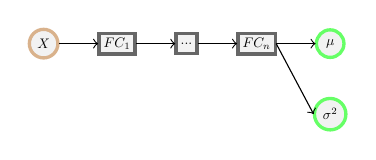
\begin{tikzpicture}[scale=0.5, transform shape,
roundnode/.style={circle, draw=brown!60, fill=black!5, very thick, minimum size=7mm},
roundnodey/.style={circle, draw=green!60, fill=black!5, very thick, minimum size=7mm},
squarednode/.style={rectangle, draw=black!60, fill=black!5, very thick, minimum size=5mm},
]
%Nodes
\node[roundnode]      (X)                             {$X$};
\node[squarednode]      (FC1)                      [right=of X]        {$FC_1$};
\node[squarednode]      (FCmiddle)             [right=of FC1]        {...};
\node[squarednode]      (FCn)                      [right=of FCmiddle]        {$FC_n$};
\node[roundnodey]      (mean)                             [right=of FCn] {$\mu$};
\node[roundnodey]      (variance)                             [below=of mean] {$\sigma^2$};

%Lines
\draw[->] (X.east) -- (FC1.west);
\draw[->] (FC1.east) -- (FCmiddle.west);
\draw[->] (FCmiddle.east) -- (FCn.west);
\draw[->] (FCn.east) -- (mean.west);
\draw[->] (FCn.east) -- (variance.west);
\end{tikzpicture}
\caption{Architecture of a single neural network.}
\label{fig:undividedarchitecture}
\end{figure}

\begin{itemize}
\item Training can be done in parallel.
% \item They are reinitialized at every SMBO step.
\item Loss function used to train the neural networks ($\sigma^2$ is variance and $\mu$ is the mean):
\end{itemize}

$$
L_{de} = -\log p(y | x) = \frac{\log \sigma^2 }{2} + \frac{(y - \mu)^2}{2\sigma^2} + \text{constant}
$$

\end{frame}

\begin{frame}[t]{FSBO}
FSBO - Few Shot Bayesian Optimization.
\begin{itemize}
\item It is a state-of-the-art transfer HPO method.
\item Formulates HPO problem as a few shot learning task.
\item Uses deep kernels as surrogates which are of the form:
$$
k(\phi(\textbf{x}, \textbf{w})  ,   \phi(\textbf{x'}, \textbf{w}) |  \mathbf{\theta})
$$
where $\textbf{x}$ and $\textbf{x'}$ are HP configurations. $\mathbf{\theta}$ and $\textbf{w}$ are parameters of kernel $k$ and the neural network $\phi$ respectively.

%\item The following are done in chronological steps
%\begin{itemize}
%\item Meta-training using existing metadata.
%\item Fine-tuning for a few epochs, i.e., few-shot learning.
%\end{itemize}
\item The loss function maximizes the following log probability
$$
\log p( \textbf{y}^{(1)}...\textbf{y}^{(T)} | \textbf{X}^{(1)}...\textbf{X}^{(T)}, \mathbf{\theta}, \textbf{w})
$$

\end{itemize}

\end{frame}

\section{Proposed Method: Ranking Losses}

\begin{frame}
\centering
\LARGE{Proposed Method: Ranking Losses}
\end{frame}

\begin{frame}[t]{Understanding Ranking}
Consider a set:
$$
\mathbb{A} = \{a_1,  a_2,  a_3, ... ,  a_n\}
$$

\begin{itemize}
\item Ranking means ordering elements of set $\mathbb{A}$.
\item We consider that lower rank is better than higher rank,  hence
$$
\texttt{Rank}(a_i) < \texttt{Rank}(a_j) \iff a_i  \succ a_j
$$
\end{itemize}

Ranking can be divided into the following components:
\begin{itemize}
\item Obtaining relevance scores of objects in the set $\mathbb{A}$.
\item Sorting objects based on relevance scores.
\end{itemize}

Since sorting is not differentiable trivially,  we only model the scoring function $s$ using an ML model.

$$
s : \mathbb{A} \mapsto \mathbb{R}
$$

\end{frame}

\begin{frame}[t]{Understanding Ranking Losses}

Consider that data is given in the following format:

\begin{table} [ht]
\centering
\begin{tabular}{ | c | c | c | }
  \toprule
  Instance & Object Set & Ground Truth \\ \midrule
% \hline \hline
  1 & $\{a_1, a_2, a_3, ... , a_{10}\}$  & $\{y_1, y_2, y_3, ... , y_{10}\}$  \\
  2 & $\{a'_1, a'_2, a'_3, ... , a'_{15}\}$ & $\{y'_1, y'_2, y'_3, ... , y'_{15}\}$  \\
  3 & $\{a''_1, a''_2, a''_3, ... , a''_{7}\}$ & $\{y''_1, y''_2, y''_3, ... , y''_{7}\}$  \\
  ... & $\{...\}$ & $\{...\}$ \\
  \bottomrule
\end{tabular}
\caption{Data used to train a scoring function.}
\label {tab:dataformat}
\end{table}

How do learn the scoring function $s$?
\begin{itemize}
\item Use a parametrized model $s_{\theta}$.
\item Use a (ranking) loss function to get the optimum $\theta^*$.
\end{itemize}

\end{frame}


\begin{frame}[t]{Understanding Ranking Losses}
Types of ranking:
\begin{itemize}
\item \textbf{Pointwise} - The model directly predicts the rank and not the score.
\item \textbf{Pairwise} - The model predicts which of the 2 inputs is better.
\item \textbf{Listwise} - Deals with a full set as 1 instance.
\end{itemize}

Types of Ranking Losses:
\begin{itemize}
\item
$
L_{\texttt{pointwise}} : s(\mathbb{A}) \times \mathbb{Y} \mapsto \mathbb{R}
$

\item
$
L_{\texttt{pairwise}} : s(\mathbb{A})_1 \times s(\mathbb{A})_2 \times \mathbb{Y}_1 \times \mathbb{Y}_2 \mapsto \mathbb{R}
$

\item
$
L_{\texttt{listwise}} : s(\mathbb{A})_1 \times s(\mathbb{A})_2 ...  s(\mathbb{A})_{n} \times \mathbb{Y}_1 \times \mathbb{Y}_2 \times ...  \mathbb{Y}_{n} \mapsto \mathbb{R}
$

\end{itemize}

\end{frame}

\begin{frame}[t]{Subset Regression: Pointwise Loss}
Basic idea:~\cite{subsetregressionpaper}
\begin{itemize}
\item Learn the rank of the objects directly.
\item Avoid intermediate relevance score.
\item Similar to RMSE.
$$
L_{\texttt{SubsetRegression}} = \frac{1}{N} \sum\limits_{i=1}^{N} (s(a_i) - \texttt{rank}(y_i))^2
$$
\end{itemize}

% Given a batch of size $N$ containing objects $a_i$ and their corresponding ground truth values $y_i$ such that $0 \leq i \leq N$,  the loss function is:

For example,  ranking for the following ground truth values is, 
$$
\{y_1 = 0.8, y_2 = 0.9, y_3 = 0.1\}
$$
$$
\texttt{rank}(y_1) = 2,  \texttt{rank}(y_2) = 1,  \texttt{rank}(y_3) = 3
$$

\end{frame}

\begin{frame}[t]{RankNet: Pairwise Loss}

\begin{itemize}
\item Classify the 2 input objects.
\item Answer the question: which object is better?
\item From all possible pairs of inputs $\{s(a_1), s(a_2), y_1, y_2\}$,  calculate loss.
$$
L_{\texttt{RankNet}} = \texttt{C.E.Loss} = -P^*\log P - (1 - P^*)\log(1-P)
$$
where $P$ and $P^*$ are given by:
$$
P(a_1 \succ a_2) = \frac{e^{s(a_1) - s(a_2)}}{1 + e^{s(a_1) - s(a_2)} }
$$
$$
P^*(a_1 \succ a_2) =
\begin{cases}
      1 & \text{if} \quad y_1 \geq y_2 \\
      0 &  \text{otherwise}
\end{cases}       
$$

Basically,  RankNet loss is the binary cross entropy loss.
\end{itemize}

% Loss calculation steps:
% \begin{itemize}
% \item Consider we are given $\{a_1, a_2, a_3..., a_n\}$ to rank.
% \item Scores of all the objects are calculated $\{s(a_1), s(a_2), s(a_3)..., s(a_n)\}$.
% \item 
% \end{itemize}

\end{frame}


\begin{frame}[t]{ListMLE: Listwise Loss}
ListMLE~\cite{listmlepaper} stands for List Maximum Likelihood Estimation.
The basic idea is:
\begin{itemize}
\item Use the whole set/list of objects as a learning instance.
\item Predict the scores of all objects using the scoring function $s$.
\item Find the "distance" between the predicted scores and the ground truth.
\item Reducing this "distance" amounts to optimization.
\end{itemize}

\textbf{Finding Distance}:

Probability of selecting an item
$$
P = \frac{\phi(s(a))}{\Sigma_i \phi(s(a_i))} 
$$
where $\phi$ is a strictly positive increasing function.
\end{frame}

\begin{frame}[t]{ListMLE: Listwise Loss}
\textbf{Finding Distance (Continued)}:

If $\pi$ defines a permutation of a list,  the probability of selecting the permutation is:
$$
P_{\pi} = \prod\limits_{j=1}^{k} \frac{\phi(s(\pi_j))}{ \sum\limits_{t=j}^k \phi(s(\pi_k))}
$$

Applying log on both sides:
$$
\log P_{\pi} = \sum\limits_{j=1}^{k} \log \frac{\phi(s(\pi_j))}{ \sum\limits_{t=j}^k \phi(s(\pi_k))}
$$

\end{frame}


\begin{frame}[t]{ListMLE: Listwise Loss}
\textbf{Finding Distance (Continued)}:
Let $\pi^*$ be the ground truth permutation. The probability of selecting $\pi^*$ is:
$$
\log P_{\pi^*} = \sum\limits_{j=1}^{k} \log \frac{\phi(s(\pi^*_j))}{ \sum\limits_{t=j}^k \phi(s(\pi^*_k))}
$$

The distance metric is given by
$$
L_{mle} = - \log P_{\pi^*}
$$
and hence
$$
L_{mle} = -  \sum\limits_{j=1}^{k} \log \frac{\phi(s(\pi^*_j))}{ \sum\limits_{t=j}^k \phi(s(\pi^*_k))}
$$

\end{frame}

\begin{frame}[t]{Weighted ListMLE}
\begin{itemize}
\item In SMBO,  it is more important to rank the first HP configuration than the last.
\item Hence,  using a weighting strategy during the calculation of distance metric makes sense.
\end{itemize}

If $c(j)$ gives the weight of the position $j$, then the loss becomes~\cite{TRLWO} -
$$
L_{mle} = -  \sum\limits_{j=1}^{k} c(j) \log \frac{\phi(s(\pi^*_j))}{ \sum\limits_{t=j}^k \phi(s(\pi^*_k))}
$$

\end{frame}

\begin{frame}[t]{Weighting Strategy}
3 different weighting strategies:
\begin{itemize}
\item Inverse linear weighting given by $c(j) = \frac{1}{j}$.
\item Inverse logarithmic weighting given by $c(j) = \frac{1}{\log (j+1)}$.
\item Position dependent ranking (scaled by 50 here) given by $c(j) = \frac{k - j + 1}{\Sigma_{t=1}^k t}$ (Chen et. al).
\end{itemize}

\begin{figure}[htb]
  \centering
    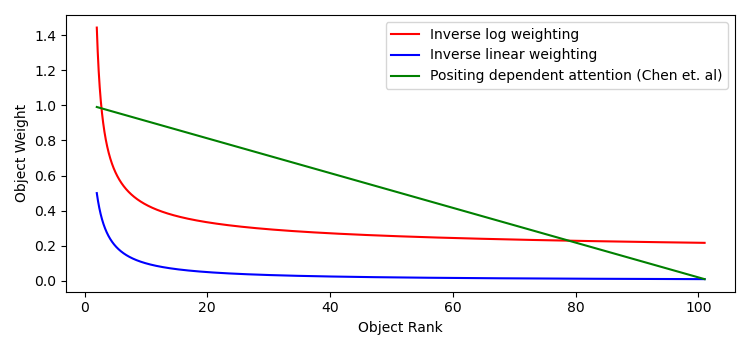
\includegraphics[scale=0.3]{images/weightingfunctions}
    \caption{Different Weighting Functions.}
    \label{fig:weightingfunctions}
\end{figure}

\end{frame}





\section{Proposed Method: Surrogate Design}

\begin{frame}

\centering
\LARGE{Proposed Method: Surrogate Design}

\end{frame}

\begin{frame}[t]{Basic Ranker}

A basic ranker is a Deep Neural Network that outputs a score and its corresponding rank.

\begin{figure}[htb]
\centering
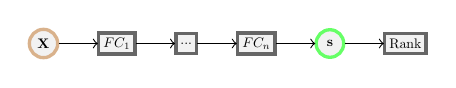
\begin{tikzpicture}[scale=0.50, transform shape,
roundnode/.style={circle, draw=brown!60, fill=black!5, very thick, minimum size=7mm},
roundnodey/.style={circle, draw=green!60, fill=black!5, very thick, minimum size=7mm},
squarednode/.style={rectangle, draw=black!60, fill=black!5, very thick, minimum size=5mm},
]
%Nodes
\node[roundnode]      (X)                             {$\textbf{X}$};
\node[squarednode]      (FC1)                      [right=of X]        {$FC_1$};
\node[squarednode]      (FCmiddle)             [right=of FC1]        {...};
\node[squarednode]      (FCn)                      [right=of FCmiddle]        {$FC_n$};
\node[roundnodey]      (y)                             [right=of FCn] {$\textbf{s}$};
\node[squarednode]      (Rank)                      [right=of y]        {Rank};

%Lines
\draw[->] (X.east) -- (FC1.west);
\draw[->] (FC1.east) -- (FCmiddle.west);
\draw[->] (FCmiddle.east) -- (FCn.west);
\draw[->] (FCn.east) -- (y.west);
\draw[->] (y.east) -- (Rank.west);
\end{tikzpicture}
\caption{Basic ranker.}
\label{fig:basicScoringModel}
\end{figure}

Given a set of inputs $\textbf{X}$,  the ranker outputs the following values
\begin{itemize}
\item Output (or) relevance scores of input elements. The values are in the \textbf{Output Space}.
\item Ranks of the input elements. The values are in the \textbf{Ranking Space}.
\end{itemize}

Note:
\begin{itemize}
\item Normal Loss functions work in the Output Space.
\item Ranking Loss functions work in the Ranking Space.
\end{itemize}

\end{frame}


\begin{frame}[t]{Basic Ranker}

A basic ranker is a Deep Neural Network that outputs a score and its corresponding rank.

\begin{figure}[htb]
\centering
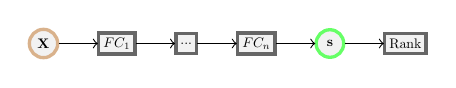
\begin{tikzpicture}[scale=0.50, transform shape,
roundnode/.style={circle, draw=brown!60, fill=black!5, very thick, minimum size=7mm},
roundnodey/.style={circle, draw=green!60, fill=black!5, very thick, minimum size=7mm},
squarednode/.style={rectangle, draw=black!60, fill=black!5, very thick, minimum size=5mm},
]
%Nodes
\node[roundnode]      (X)                             {$\textbf{X}$};
\node[squarednode]      (FC1)                      [right=of X]        {$FC_1$};
\node[squarednode]      (FCmiddle)             [right=of FC1]        {...};
\node[squarednode]      (FCn)                      [right=of FCmiddle]        {$FC_n$};
\node[roundnodey]      (y)                             [right=of FCn] {$\textbf{s}$};
\node[squarednode]      (Rank)                      [right=of y]        {Rank};

%Lines
\draw[->] (X.east) -- (FC1.west);
\draw[->] (FC1.east) -- (FCmiddle.west);
\draw[->] (FCmiddle.east) -- (FCn.west);
\draw[->] (FCn.east) -- (y.west);
\draw[->] (y.east) -- (Rank.west);
\end{tikzpicture}
\caption{Basic ranker.}
\label{fig:basicScoringModel}
\end{figure}

Advantages of working in the ranking space:
\begin{itemize}
\item Ranking is agnostic to affine transformations of score i.e $\alpha * s + \beta$ where $\alpha, \beta \in \mathbb{R}$.
\item Larger target output space leads to easier convergence/learning.
\item Ranks from different rankers can be combined easily.
\end{itemize}

\end{frame}

\begin{frame}[t]{Ensemble of Basic Rankers}

\begin{figure}[htb]
\centering
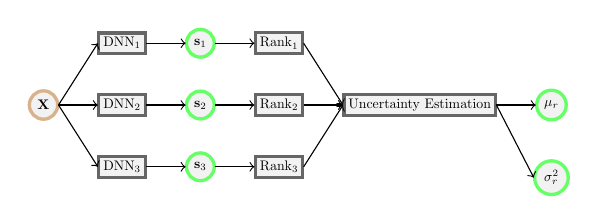
\begin{tikzpicture}[scale=0.50, transform shape,
roundnode/.style={circle, draw=brown!60, fill=black!5, very thick, minimum size=7mm},
roundnodey/.style={circle, draw=green!60, fill=black!5, very thick, minimum size=7mm},
squarednode/.style={rectangle, draw=black!60, fill=black!5, very thick, minimum size=5mm},
]
%Nodes
\node[roundnode]          (X)                                           {$\textbf{X}$};
\node[squarednode]      (DNN2)                      [right=of X]        {DNN$_2$};
\node[squarednode]      (DNN1)                      [above=of DNN2]                    {DNN$_1$};
\node[squarednode]      (DNN3)                      [below=of DNN2]                    {DNN$_3$};
\node[roundnodey]        (y1)                             [right=of DNN1] {$\textbf{s}_1$};
\node[roundnodey]        (y2)                             [right=of DNN2] {$\textbf{s}_2$};
\node[roundnodey]        (y3)                             [right=of DNN3] {$\textbf{s}_3$};
\node[squarednode]      (Rank1)                             [right=of y1] {Rank$_1$};
\node[squarednode]      (Rank2)                             [right=of y2] {Rank$_2$};
\node[squarednode]      (Rank3)                             [right=of y3] {Rank$_3$};
\node[squarednode]      (UncertaintyEstimation)                             [right=of Rank2] {Uncertainty Estimation};
\node[roundnodey]        (mus)                             [right=of UncertaintyEstimation] {$\mu_r$};
\node[roundnodey]        (sigmas)                             [below=of mus] {$\sigma^2_r$};

%Lines
\draw[->] (X.east) -- (DNN1.west);
\draw[->] (X.east) -- (DNN2.west);
\draw[->] (X.east) -- (DNN3.west);
\draw[->] (DNN1.east) -- (y1.west);
\draw[->] (DNN2.east) -- (y2.west);
\draw[->] (DNN3.east) -- (y3.west);
\draw[->] (y1.east) -- (Rank1.west);
\draw[->] (y2.east) -- (Rank2.west);
\draw[->] (y3.east) -- (Rank3.west);
\draw[->] (Rank1.east) -- (UncertaintyEstimation.west);
\draw[->] (Rank2.east) -- (UncertaintyEstimation.west);
\draw[->] (Rank3.east) -- (UncertaintyEstimation.west);
\draw[->] (UncertaintyEstimation.east) -- (mus.west);
\draw[->] (UncertaintyEstimation.east) -- (sigmas.west);

\end{tikzpicture}
\caption{Ensemble of Basic Rankers.}
\label{fig:proposeModelUncertainty}
\end{figure}

\begin{itemize}
\item Ensemble of Basic rankers gives a list of ranks for every input element.
\item Gaussian uncertainty is calculated in the ranking space. The mean and standard deviation are calculated using the following formulae:
$$
\mu_r = \frac{ \sum\limits_{i=1}^{m} y_i}{m}  \;\;\;\;\;  \sigma_r =\frac{ \sum\limits_{i=1}^{m} (y_i - y_{mean})^2}{m}
$$
\end{itemize}

\end{frame}

\begin{frame}[t]{Making model context aware}

The model is made context-aware by using Deep Sets.

\begin{figure}[htb]
\centering
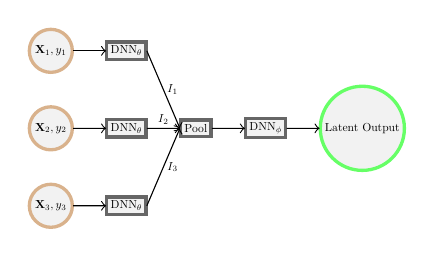
\begin{tikzpicture}[scale=0.42, transform shape,
roundnode/.style={circle, draw=brown!60, fill=black!5, very thick, minimum size=7mm},
roundnodey/.style={circle, draw=green!60, fill=black!5, very thick, minimum size=7mm},
squarednode/.style={rectangle, draw=black!60, fill=black!5, very thick, minimum size=5mm},
]
%Nodes
\node[roundnode]      (X1)                             {$\textbf{X}_1, y_1$};
\node[roundnode]      (X2)                            [below=of X1]     {$\textbf{X}_2, y_2$};
\node[roundnode]      (X3)                            [below=of X2]     {$\textbf{X}_3, y_3$};
\node[squarednode]      (phi1)                      [right=of X1]        {DNN$_{\theta}$};
\node[squarednode]      (phi2)                     [right=of X2]        {DNN$_{\theta}$};
\node[squarednode]      (phi3)                     [right=of X3]        {DNN$_{\theta}$};
\node[squarednode]      (Pool)                     [right=of phi2]     {Pool};
\node[squarednode]      (pho)                      [right=of Pool]     {DNN$_{\phi}$};
\node[roundnodey]      (LatentOutput)         [right=of pho]     {Latent Output};

%Lines
\draw[->] (X1.east) -- (phi1.west);
\draw[->] (X2.east) -- (phi2.west);
\draw[->] (X3.east) -- (phi3.west);
\draw[->] (phi1.east) -- (Pool.west)    node[midway, right] {$I_1$};
\draw[->] (phi2.east) -- (Pool.west)   node[midway, above] {$I_2$};
\draw[->] (phi3.east) -- (Pool.west)   node[midway, right] {$I_3$};
\draw[->] (Pool.east) -- (pho.west);
\draw[->] (pho.east) -- (LatentOutput.west);
\end{tikzpicture}
\caption{Deep Set Architecture.}
\label{fig:DeepSetArchitecture}
\end{figure}

\begin{itemize}
\item The architecture consists of 3 separate components: DDN$_{\theta}$,  Pool,  and DNN$_{\phi}$.
\item Pooling operator $\frac{ I_1 + I_2 + I_3}{3}$ takes care of:
\begin{itemize}
\item Permutation-Invariance constraint.
\item Set cardinality invariance constraint.
\end{itemize}
\end{itemize}

\end{frame}

\begin{frame}[t]{Making model context aware}

\begin{figure}[htb]
\centering
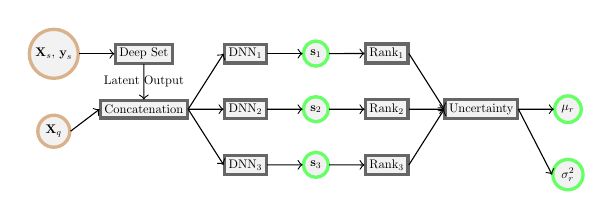
\begin{tikzpicture}[scale=0.45, transform shape,
roundnode/.style={circle, draw=brown!60, fill=black!5, very thick, minimum size=7mm},
roundnodey/.style={circle, draw=green!60, fill=black!5, very thick, minimum size=7mm},
squarednode/.style={rectangle, draw=black!60, fill=black!5, very thick, minimum size=5mm},
]
%Nodes
\node[roundnode]          (Xs)                                                     {$\textbf{X}_s$, $\textbf{y}_s$};
\node[roundnode]          (Xq)                        [below=of Xs]     {$\textbf{X}_q$};
\node[squarednode]      (DeepSet)              [right=of Xs]        {Deep Set};
\node[squarednode]      (Concatenation)             [below=of DeepSet]        {Concatenation};
\node[squarednode]      (DNN2)                      [right=of Concatenation]        {DNN$_2$};
\node[squarednode]      (DNN1)                      [above=of DNN2]                    {DNN$_1$};
\node[squarednode]      (DNN3)                      [below=of DNN2]                    {DNN$_3$};
\node[roundnodey]        (s1)                             [right=of DNN1] {$\textbf{s}_1$};
\node[roundnodey]        (s2)                             [right=of DNN2] {$\textbf{s}_2$};
\node[roundnodey]        (s3)                             [right=of DNN3] {$\textbf{s}_3$};
\node[squarednode]      (rank2)                             [right=of s2] {Rank$_2$};
\node[squarednode]      (rank3)                             [below=of rank2] {Rank$_3$};
\node[squarednode]      (rank1)                             [above=of rank2] {Rank$_1$};
\node[squarednode]      (uncertainty)                             [right=of rank2] {Uncertainty};
\node[roundnodey]        (mus)                             [right=of uncertainty] {$\mu_r$};
\node[roundnodey]        (sigmas)                             [below=of mus] {$\sigma^2_r$};

%Lines
\draw[->] (Xs.east) -- (DeepSet.west);
\draw[->] (DeepSet.south) -- (Concatenation.north) node[midway] {Latent Output};
\draw[->] (Xq.east) -- (Concatenation.west);
\draw[->] (Concatenation.east) -- (DNN1.west);
\draw[->] (Concatenation.east) -- (DNN2.west);
\draw[->] (Concatenation.east) -- (DNN3.west);
\draw[->] (DNN1.east) -- (s1.west);
\draw[->] (DNN2.east) -- (s2.west);
\draw[->] (DNN3.east) -- (s3.west);
\draw[->] (s1.east) -- (rank1.west);
\draw[->] (s2.east) -- (rank2.west);
\draw[->] (s3.east) -- (rank3.west);
\draw[->] (rank1.east) -- (uncertainty.west);
\draw[->] (rank2.east) -- (uncertainty.west);
\draw[->] (rank3.east) -- (uncertainty.west);
\draw[->] (uncertainty.east) -- (mus.west);
\draw[->] (uncertainty.east) -- (sigmas.west);

\end{tikzpicture}
\caption{Skeleton of the proposed model with Deep Sets.}
\label{fig:proposeModelDeepSets}
\end{figure}

\begin{itemize}
\item Support set, i.e., know HP configurations and their evaluations are passed through Deep Set to get a latent output.
\item The query HP configurations are concatenated with the latent output.
\item The concatenation is passed through the ensemble of \\
deep rankers.
\item During training/finetuning, losses are aggregated in the\\
 ranking space.
\end{itemize}

\end{frame}

\begin{frame}[t]{Surrogate usage}

\begin{itemize}
\item The proposed surrogate is a transfer HPO surrogate used in SMBO.
\item There are 2 stages of using it:
\begin{itemize}
\item Meta training before SMBO optimization cycle.
\item Finetuning during the SMBO optimization cycle.
\end{itemize}
\end{itemize}

\textbf{Meta-training}
\begin{itemize}
\item Goal: Learn the common characteristics of all tasks and transfer knowledge to the new task.
\item Separate surrogate is learned for each SS.
\item Concept of double sampling is used, i.e., sample the task then from the task sample the metadata.
\item Learning done using stochastic gradient descent for 5000 epochs.
\item Used ADAM optimizer with a learning rate of 0.0001. 
\end{itemize}

\end{frame}


\begin{frame}[t]{Surrogate usage}

\textbf{Finetuning}
\begin{itemize}
\item Finetuning helps improve the HPO results.
\item A full batch gradient is used with the ADAM optimizer to finetune for 1000 epochs.
\item The finetuning is restarted at every SMBO evaluation step to get better performance.
\item We use cosine annealing during the finetuning process.
\end{itemize}

\end{frame}

\begin{frame}[t]{Restarting is necessary during finetuning}

This idea is counter-intuitive because an already trained model should converge faster to a local optimum. Reasons for this observation are:
\begin{itemize}
\item Model is biased towards already seen points.
\end{itemize}

\begin{figure}[h]% [H] is so declass\'e!
\centering
\begin{minipage}{0.45\textwidth}
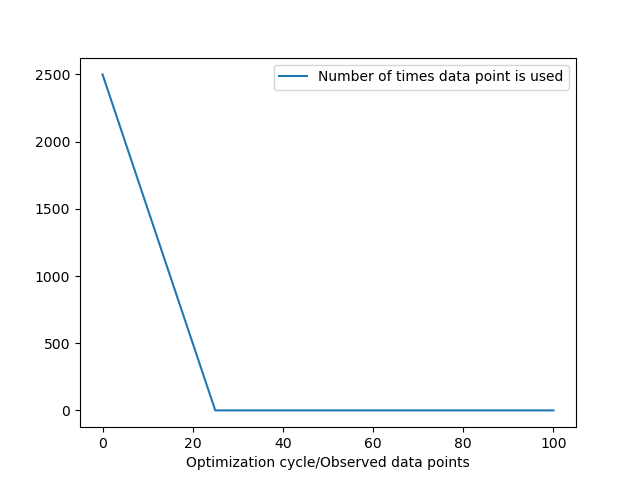
\includegraphics[width=\textwidth]{images/bias25}
\caption{Bias at $25^{th}$ optimization cycle.}
    \label{fig:bias25}
\end{minipage}\hfill
\begin{minipage}{0.45\textwidth}
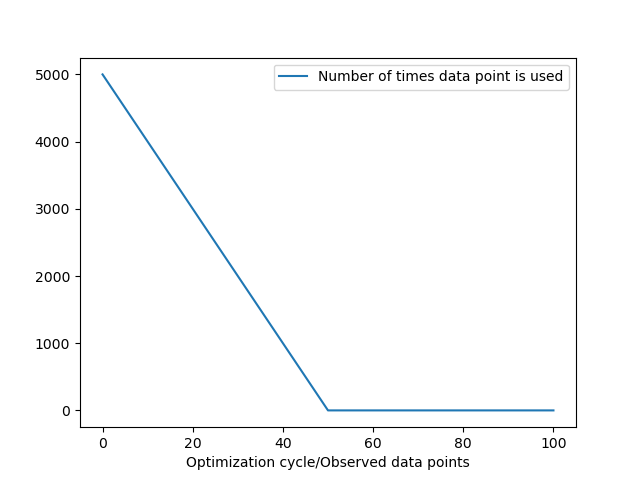
\includegraphics[width=\textwidth]{images/bias50}
\caption{Bias at $50^{th}$ optimization cycle.}
    \label{fig:bias50}
\end{minipage}\par
\end{figure}

\end{frame}

\begin{frame}[t]{Restarting is necessary during finetuning}
\begin{itemize}
\item Stubborn local minima
\begin{itemize}
\item Response surface does not change significantly with the addition of only a single data point.
\item Restarting the training can increase changes of reaching good optima.
\end{itemize} 
\end{itemize}

\begin{figure}[htb]
  \centering
    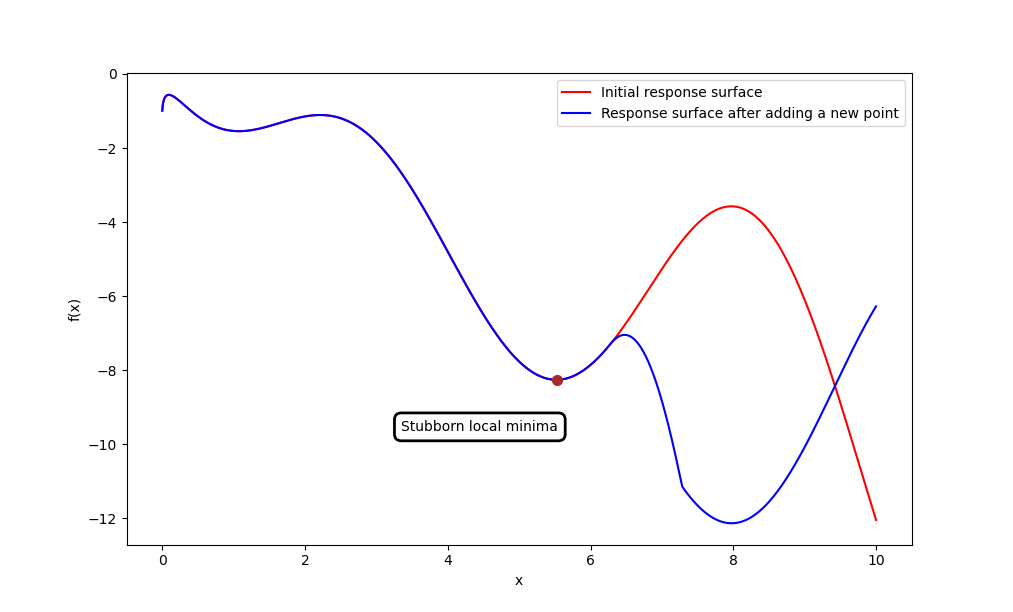
\includegraphics[scale=0.37]{images/localMinima}
    \caption{Illustration of changes in response surfaces and a stubborn local minimum.}
    \label{fig:localMinima}
\end{figure}

\end{frame}

\section{Experiments and Results}
\begin{frame}

\centering
\LARGE{Experiments and Results}

\end{frame}

\begin{frame}[t]{Q1: Which loss function is better?}

We compare the following loss function types:
\begin{itemize}
\item Regression Loss (Ref.  RMSE)
\item Pointwise ranking loss (Ref.  Subset Regression)
\item Pairwise ranking loss (Ref.  RankNet)
\item Listwise ranking loss (Ref.  ListMLE)
\end{itemize}
Baseline DE-M10-RS is used, which stands for Deep Ensemble with 10 neural networks with restart mechanism.
2 cases have to be compared separately.
\begin{itemize}
\item Non-transfer HPO
\item Transfer HPO
\end{itemize}


\end{frame}

\begin{frame}[t]{Q1: Which loss function is better? - Non transfer HPO}

\begin{figure}[h]
  \centering
    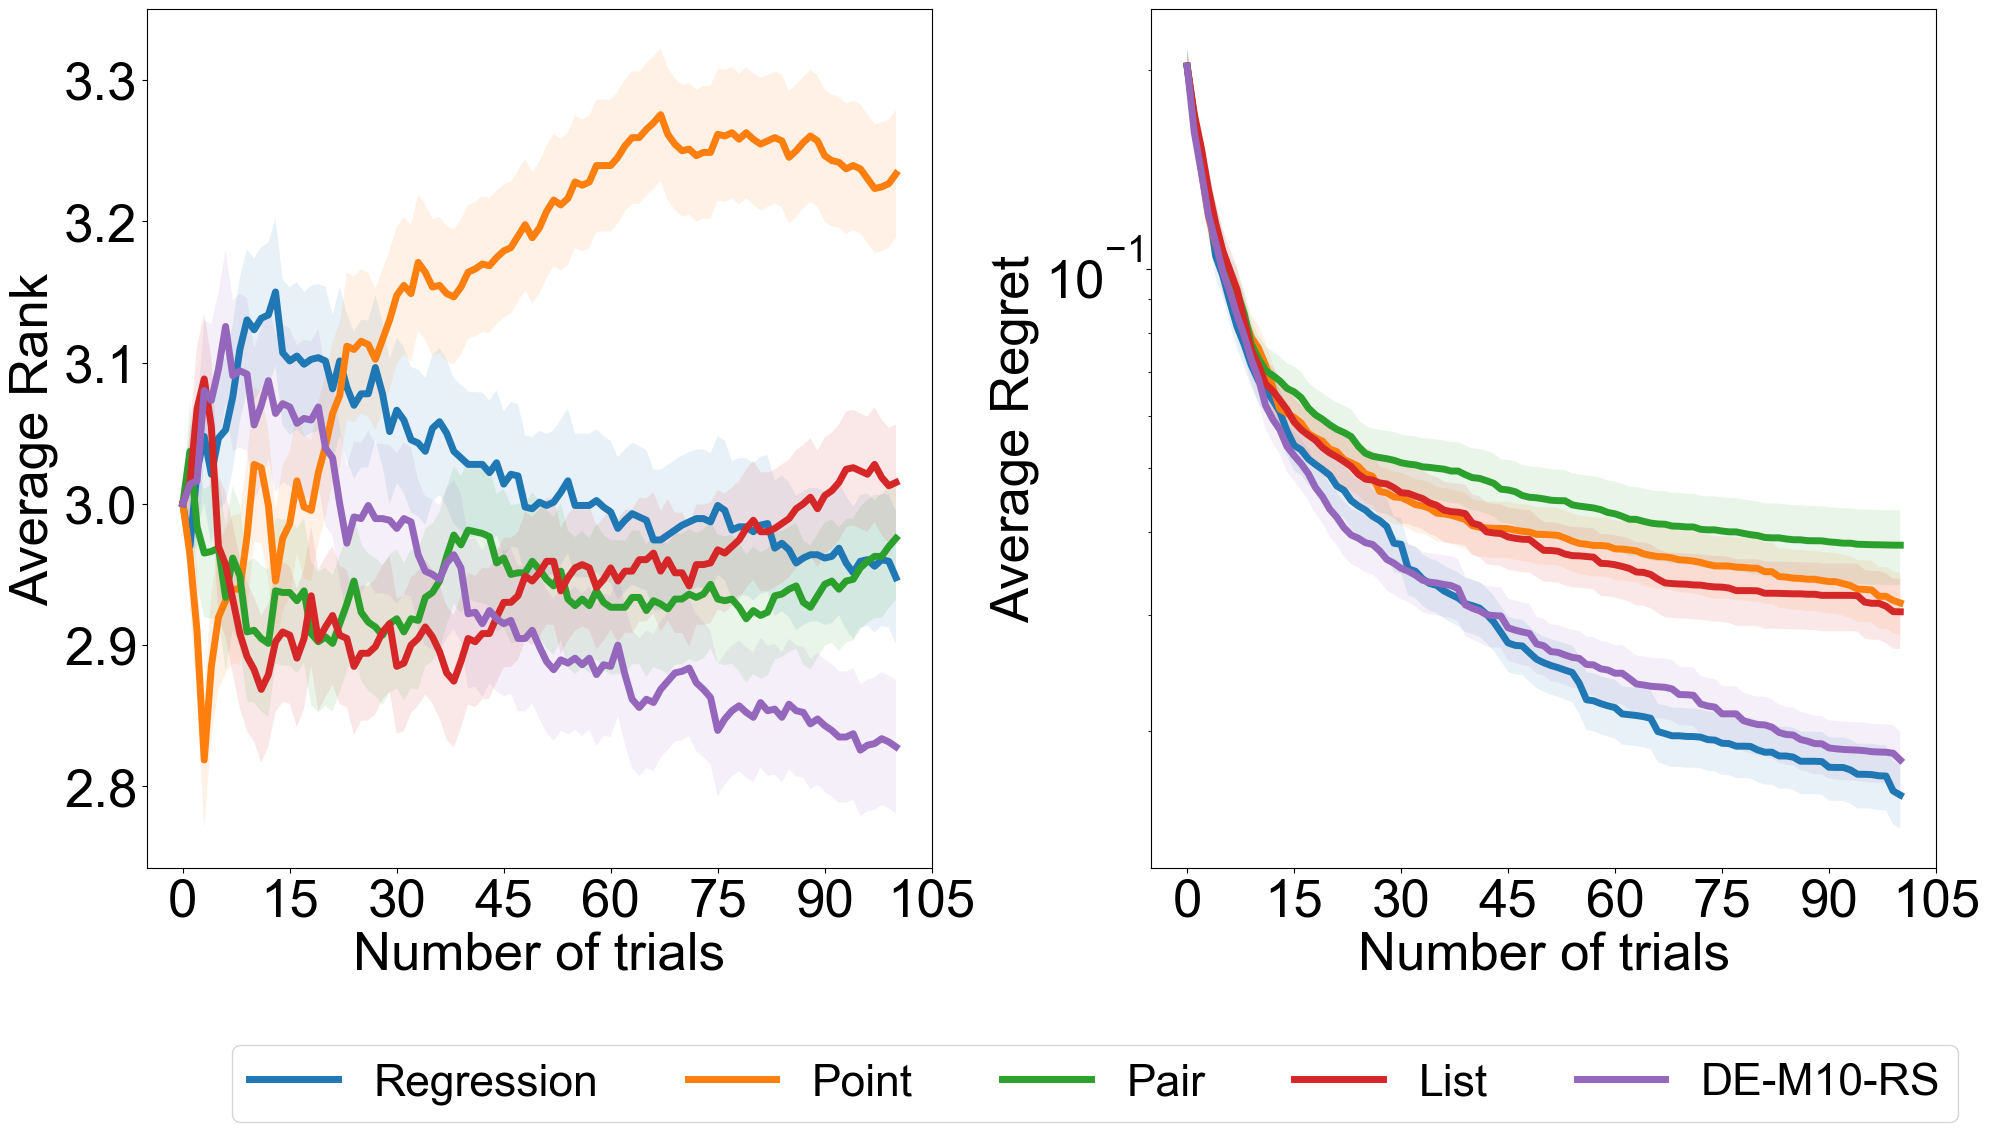
\includegraphics[scale=0.15]{images/Q1AblationNonTransfer}
    \label{fig:Q1AblationNonTransfer}
\end{figure}

\begin{figure}[h]% [H] is so declass\'e!
\centering
\begin{minipage}{0.45\textwidth}
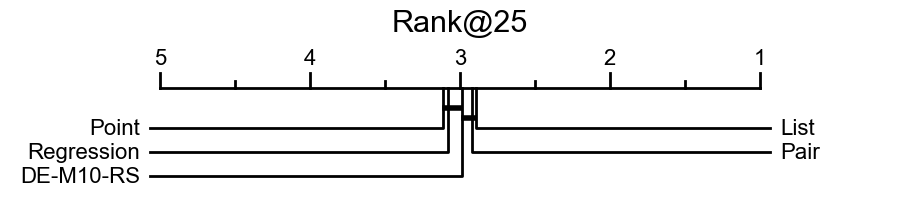
\includegraphics[width=\textwidth]{images/Q1AblationNonTransferRank@25}
\end{minipage}\hfill
\begin{minipage}{0.45\textwidth}
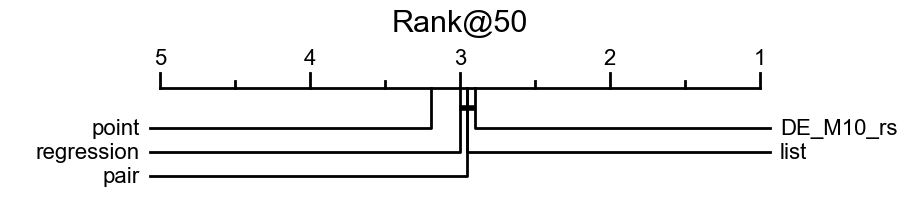
\includegraphics[width=\textwidth]{images/Q1AblationNonTransferRank@50}
\end{minipage}\par
\vskip\floatsep% normal separation between figures
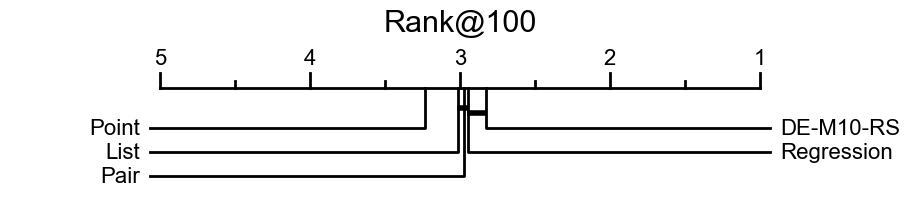
\includegraphics[width=0.45\textwidth]{images/Q1AblationNonTransferRank@100}
    \caption{Rank Graph \& Critical rank graph for non-transfer HPO.}
   \label{fig:Q1AblationNonTransferRank100}
\end{figure}

\end{frame}


\begin{frame}[t]{Q1: Which loss function is better? - Transfer HPO}

\begin{figure}[h]
  \centering
    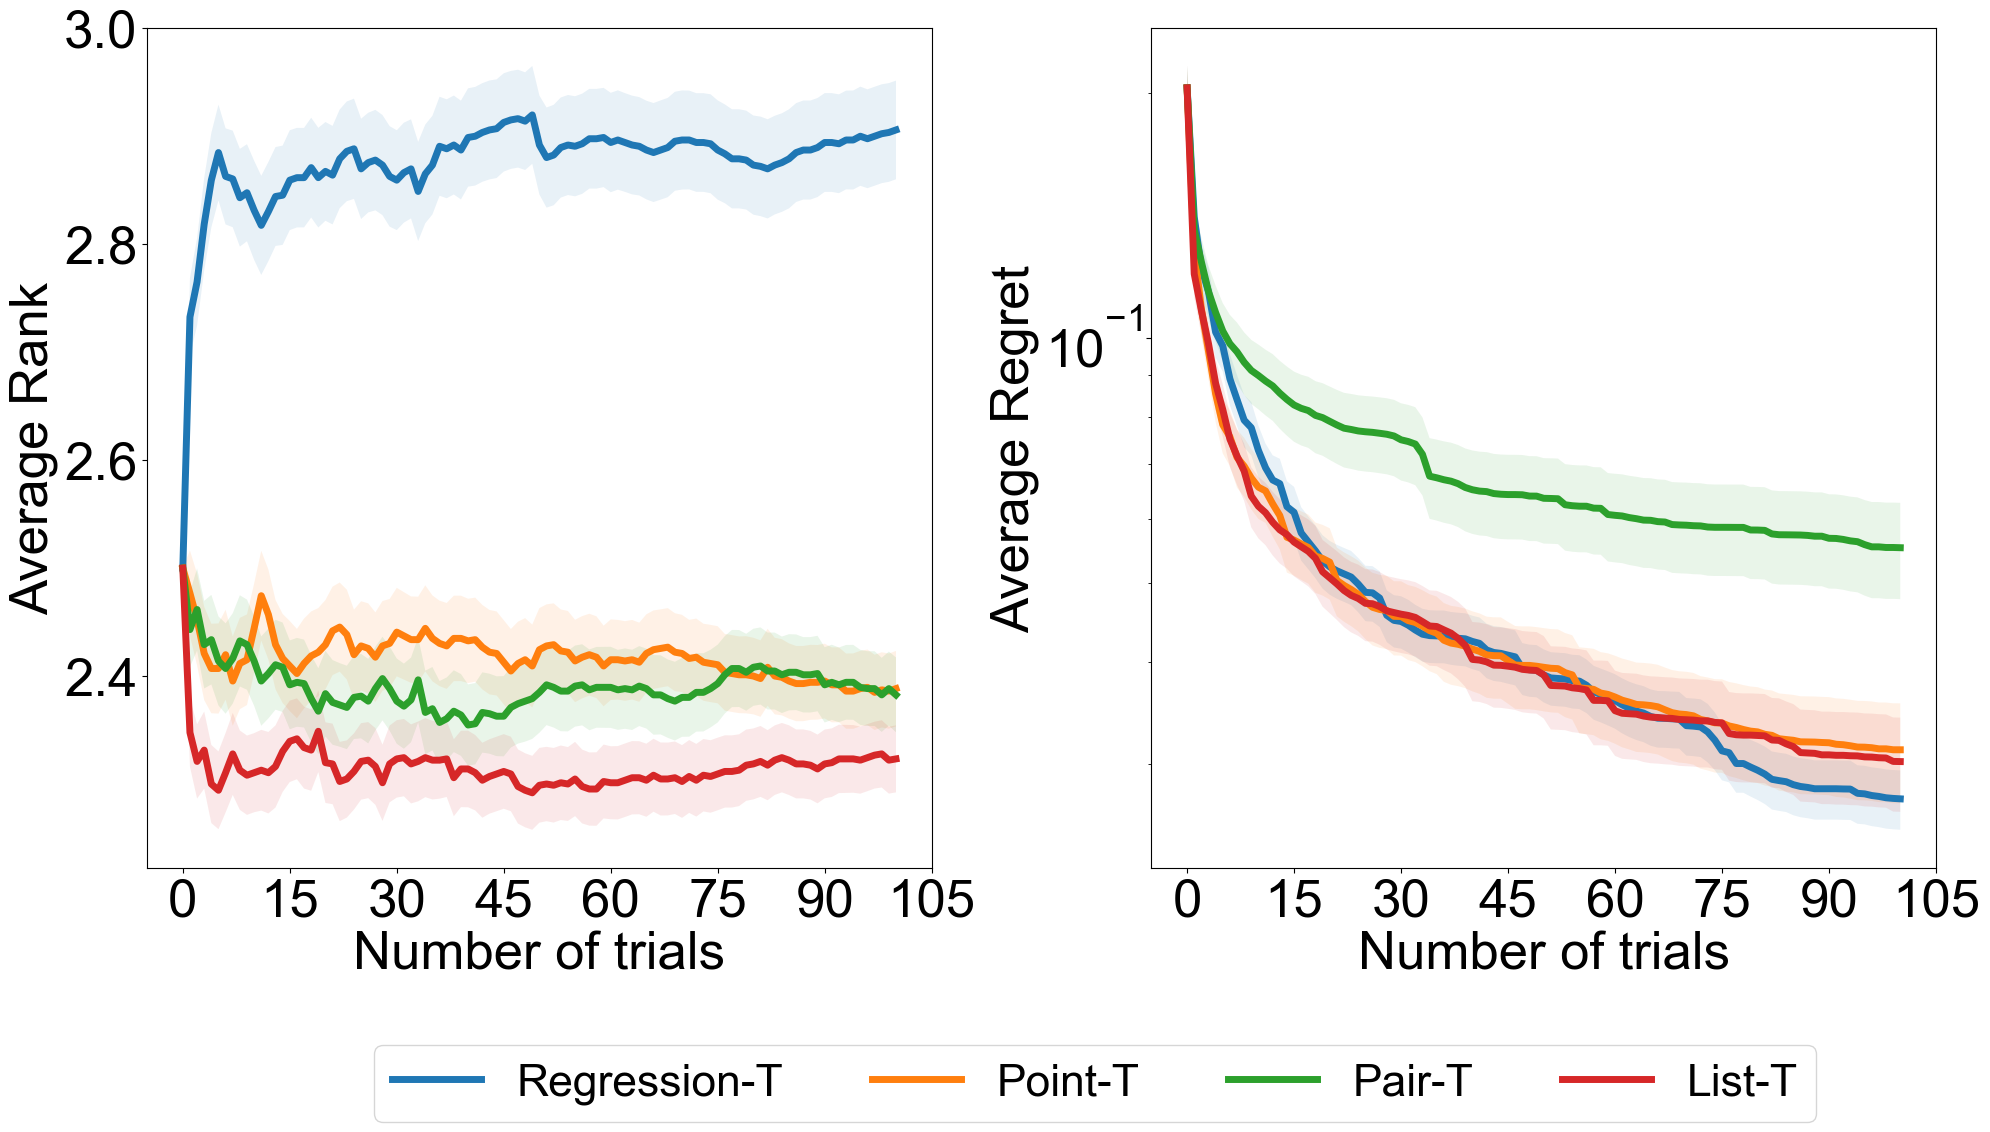
\includegraphics[scale=0.12]{images/Q1AblationTransfer} 
     \caption{Loss comparison. "T" stands for transfer.}
    \label{fig:Q1AblationTransfer}
\end{figure}

\textbf{Conclusion:  Listwise ranking loss on average performs better than other losses.}

\end{frame}

\begin{frame}[t]{Q1: Does weighting Listwise loss improve results?}
\begin{figure}[h]
  \centering
    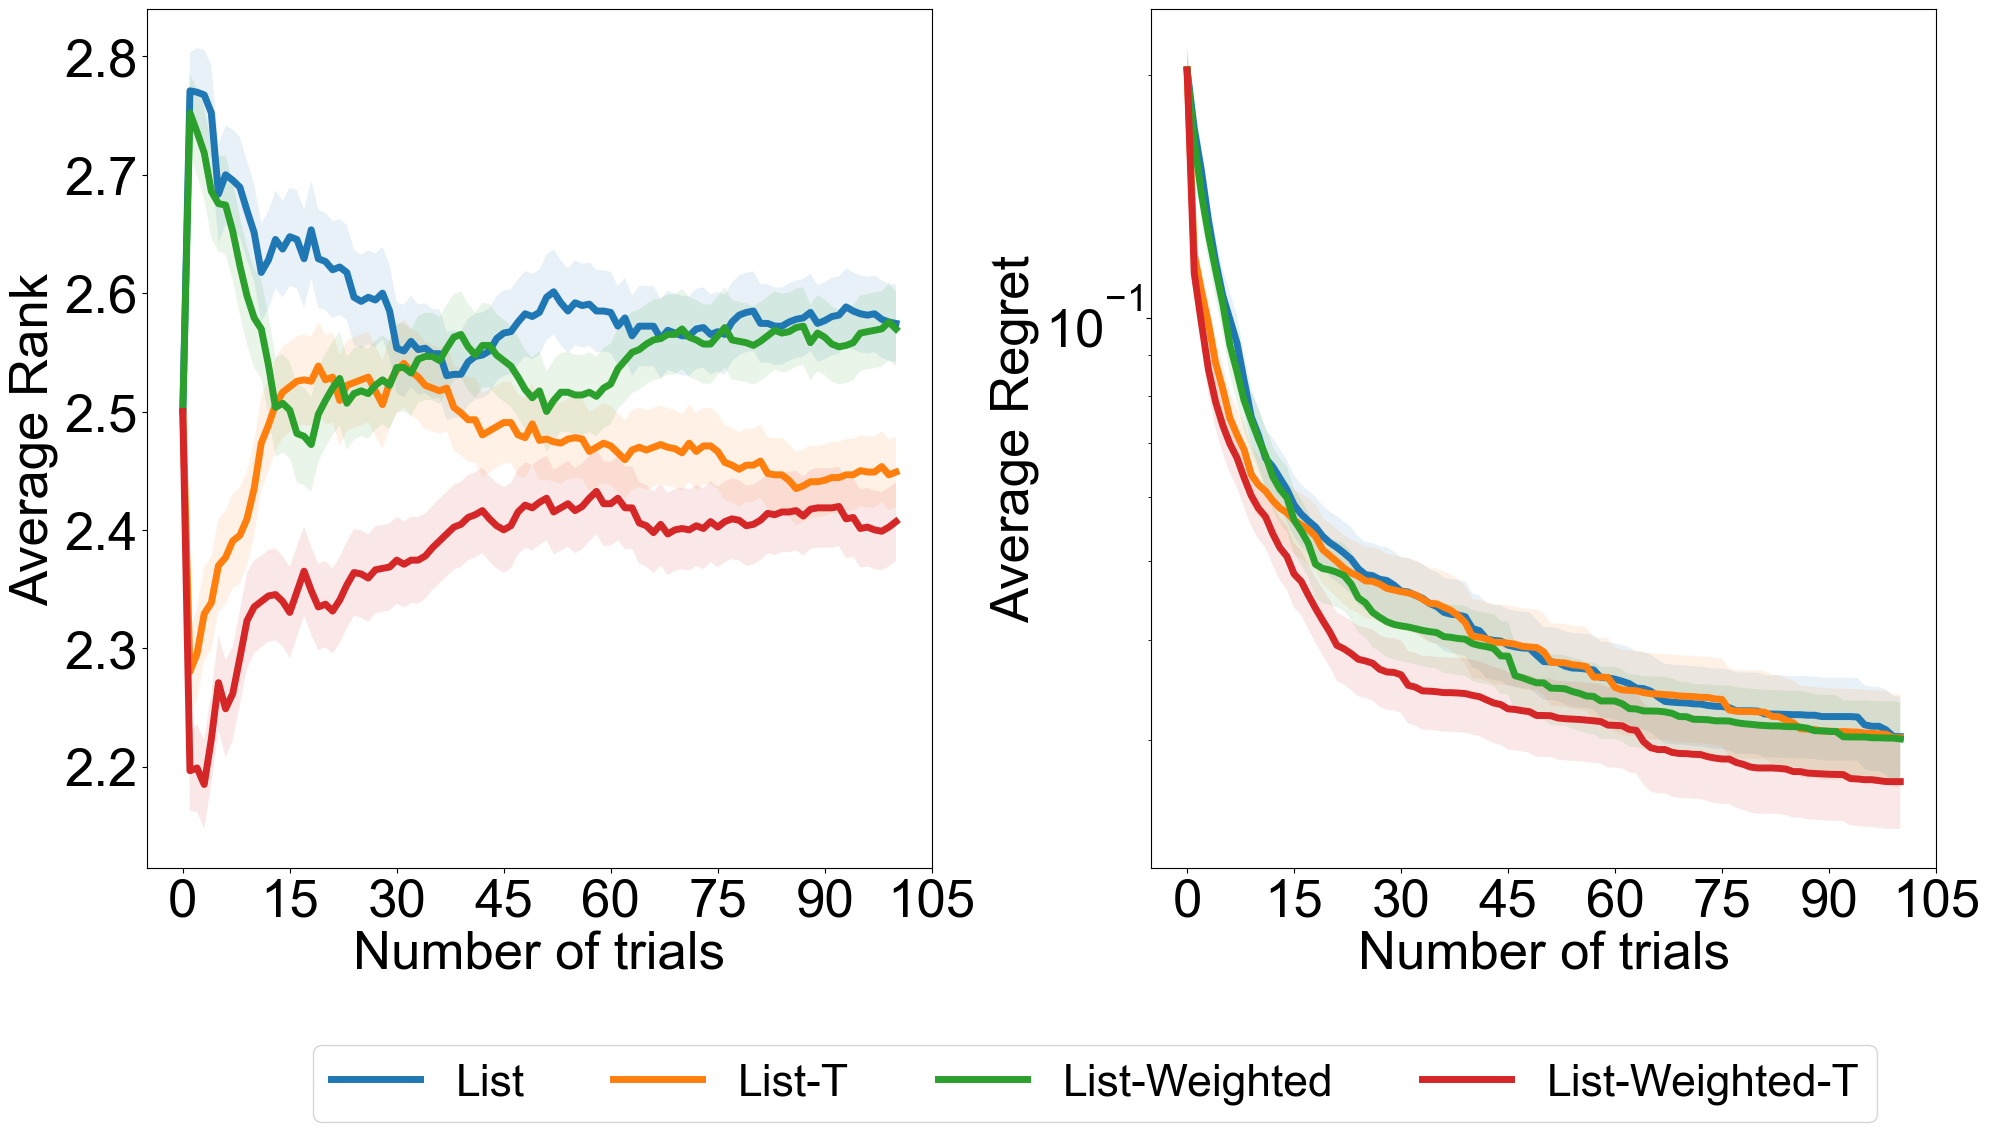
\includegraphics[scale=0.12]{images/Q2Ablation}
    \caption{Listwise losses with and without weighting.}
    \label{fig:Q2Ablation}
\end{figure}

\begin{itemize}
\item Inverse logorithmic weighting used for both the transfer and non-transfer case.
\item \textbf{Conclusion:} Weighting improves the results for both transfer and non-transfer HPO.
\end{itemize}

\end{frame}

\begin{frame}[t]{Q1: Does adding Deep Sets improve performance?}

\begin{figure}[h]
  \centering
    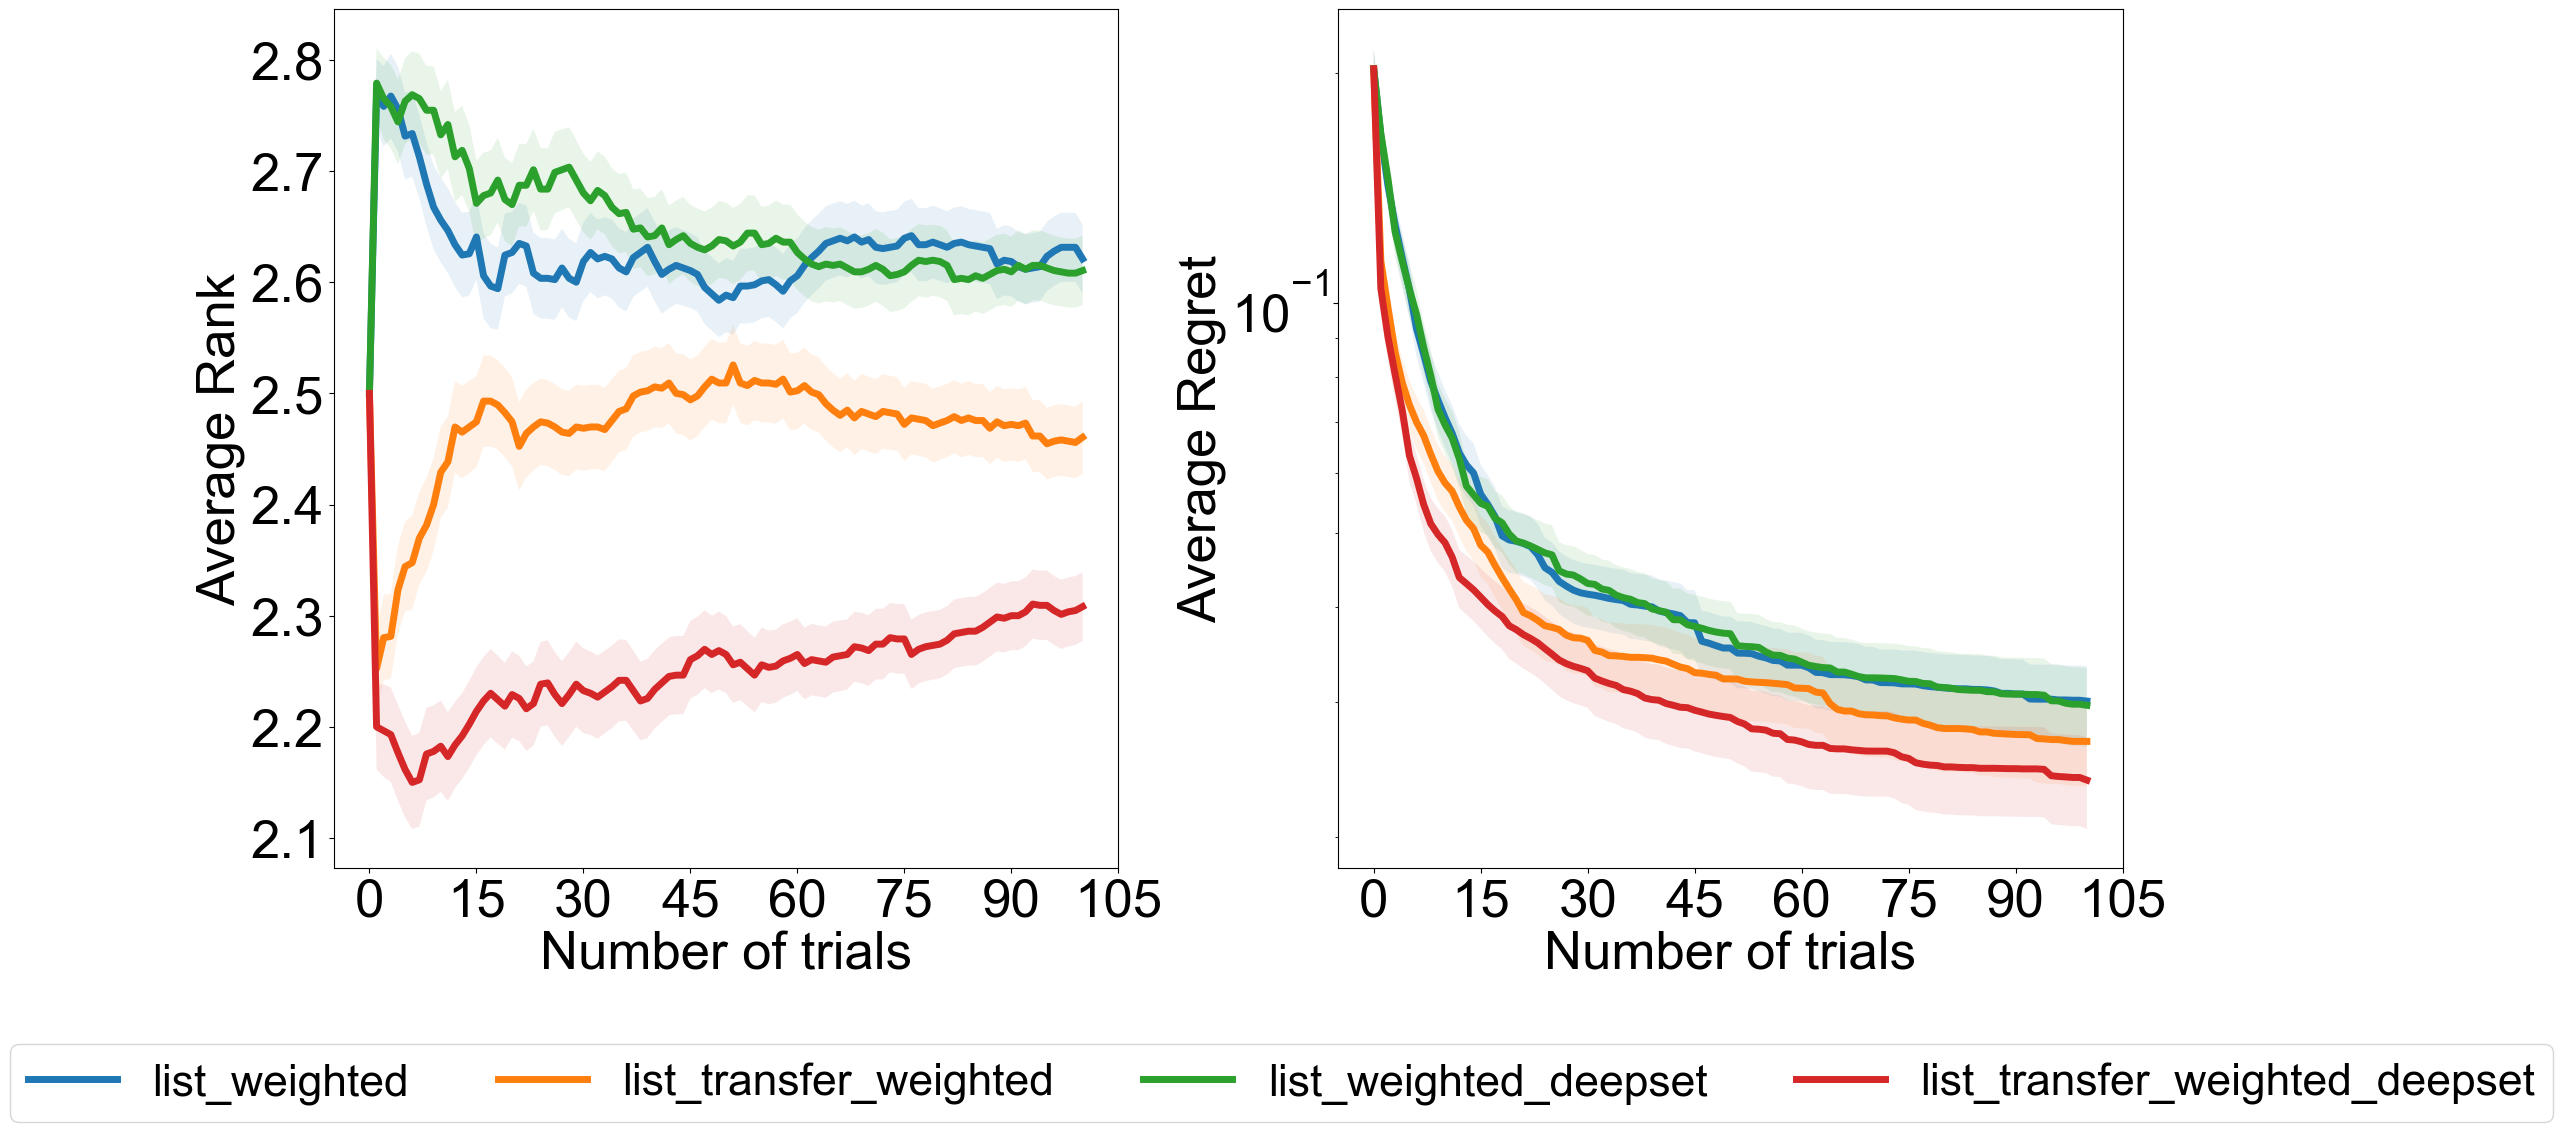
\includegraphics[scale=0.12]{images/Q3Ablation}
    \caption{Effect of adding deep sets into the architecture.}
    \label{fig:Q3Ablation}
\end{figure}

\begin{itemize}
\item 20\% of data is used as support set for both training and finetuning.
\item \textbf{Conclusion}:
\begin{itemize}
\item Non-transfer HPO results become worse.  Reason is high complexity of the model.
\item Transfer HPO results become very good in the initial steps.
\end{itemize}
\end{itemize}

\end{frame}

\begin{frame}[t]{Q1: Does finetuning improve performance?}

\begin{figure}[h]
  \centering
    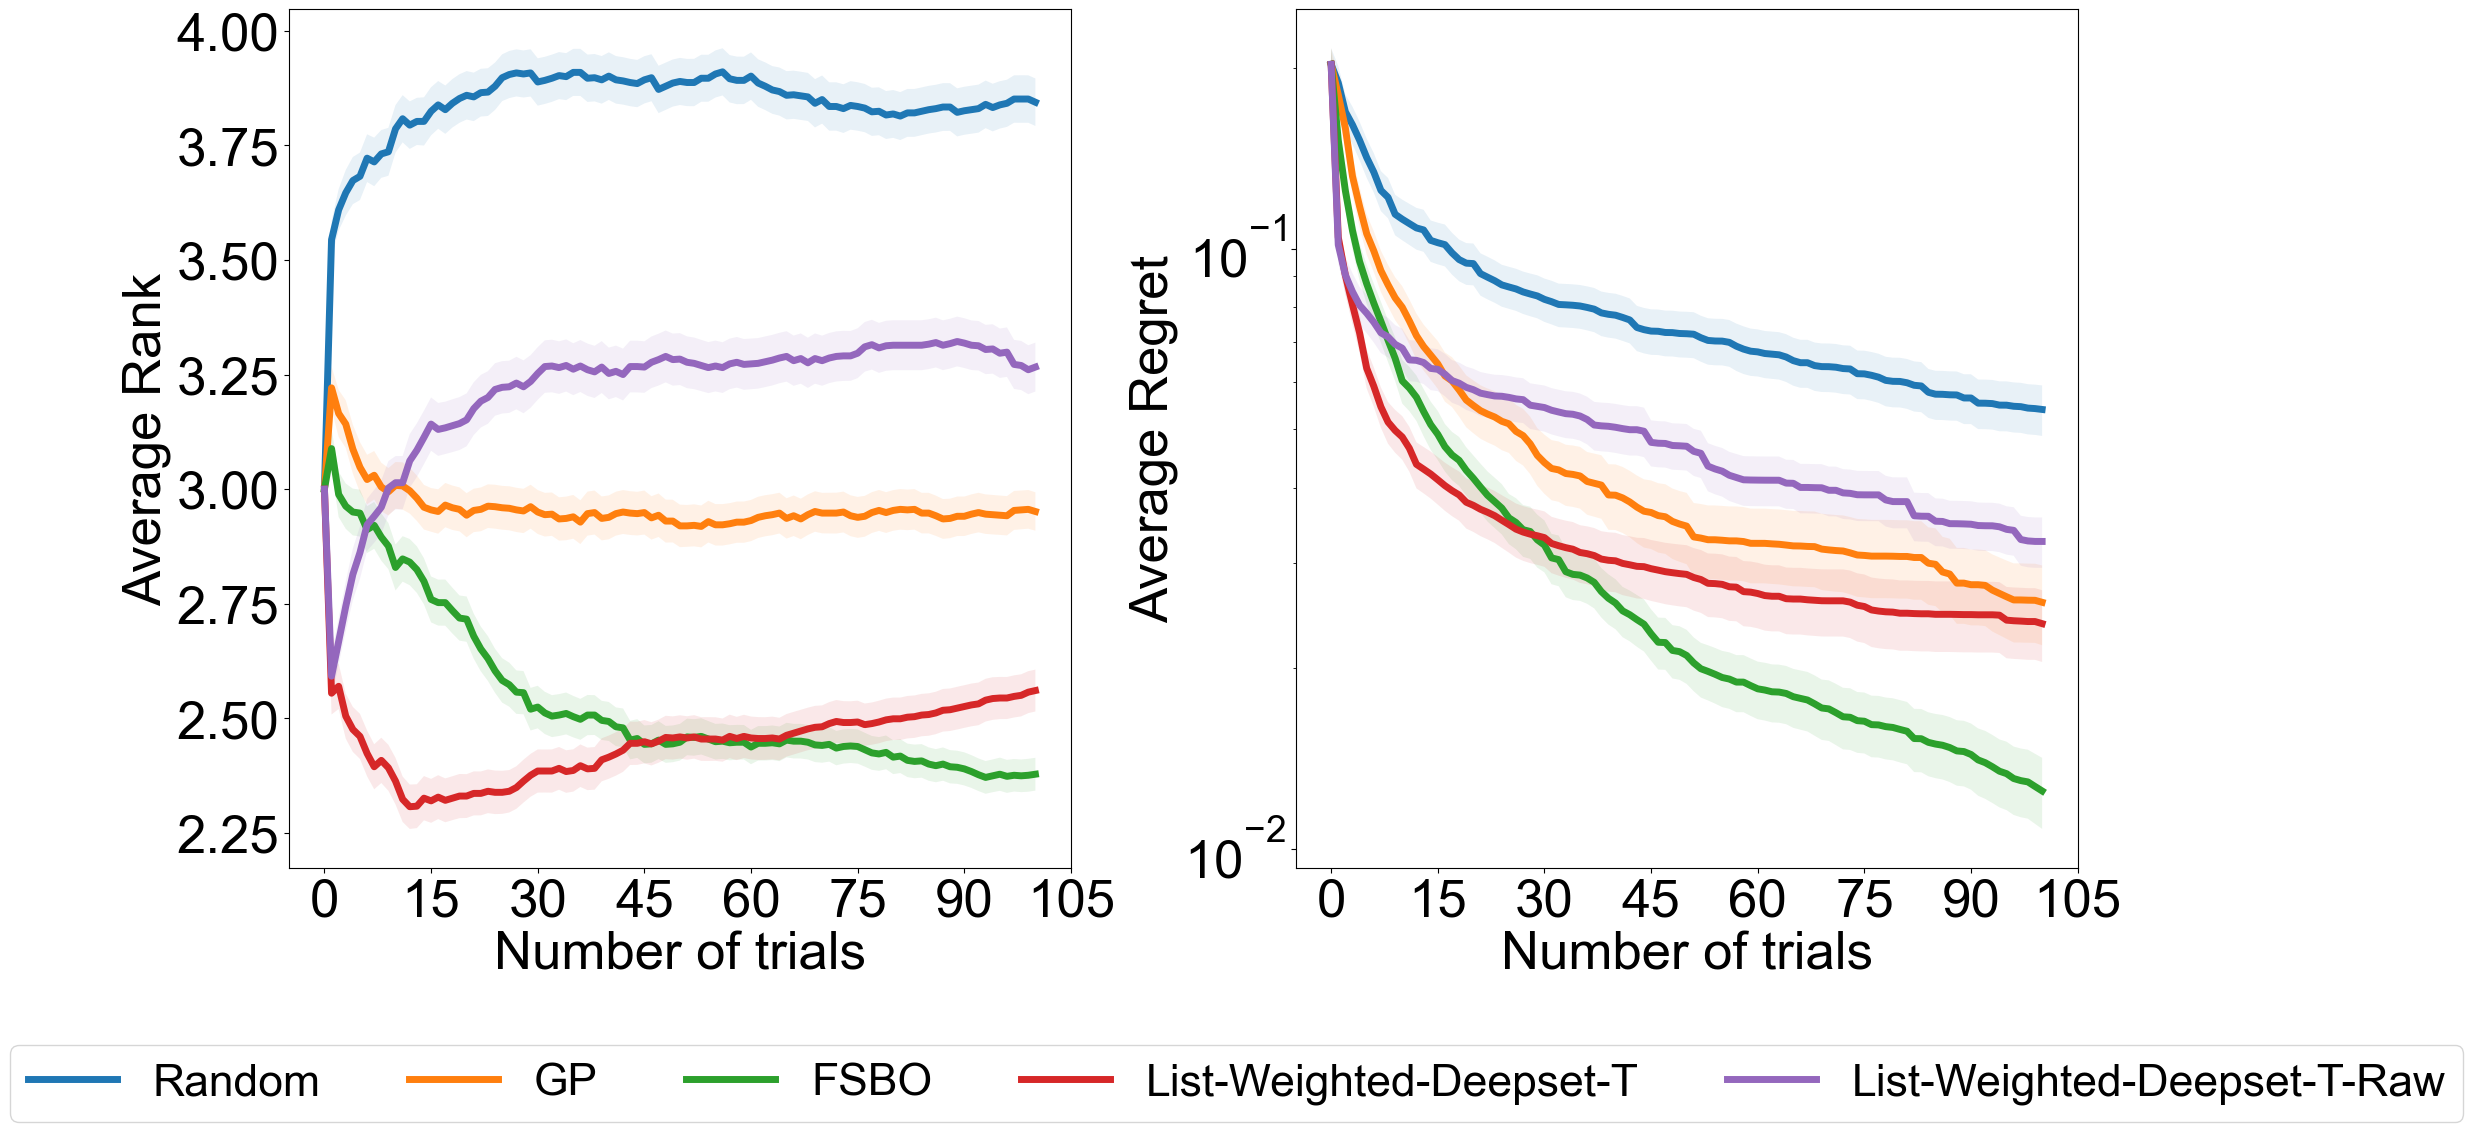
\includegraphics[scale=0.12]{images/FineTuningAblation}
    \caption{Effect of using finetuning.}
    \label{fig:FineTuningAblation}
\end{figure}

\begin{itemize}
\item Here,  "Raw" means a meta-trained model without finetuning.
\item Not doing finetuning amounts to ranking the complete list of HP configuration and evaluating it.
\item Using finetuning means learning the new context.
\item \textbf{Conclusion}:
\begin{itemize}
\item No finetuning performs well only in the first steps.
\item Finetuning is required for better long-term results.
\end{itemize}
\end{itemize}

\end{frame}


\begin{frame}[t]{Comparing with SOTA HPO models}
\textbf{Non-transfer HPO}
\begin{figure}[h]
  \centering
    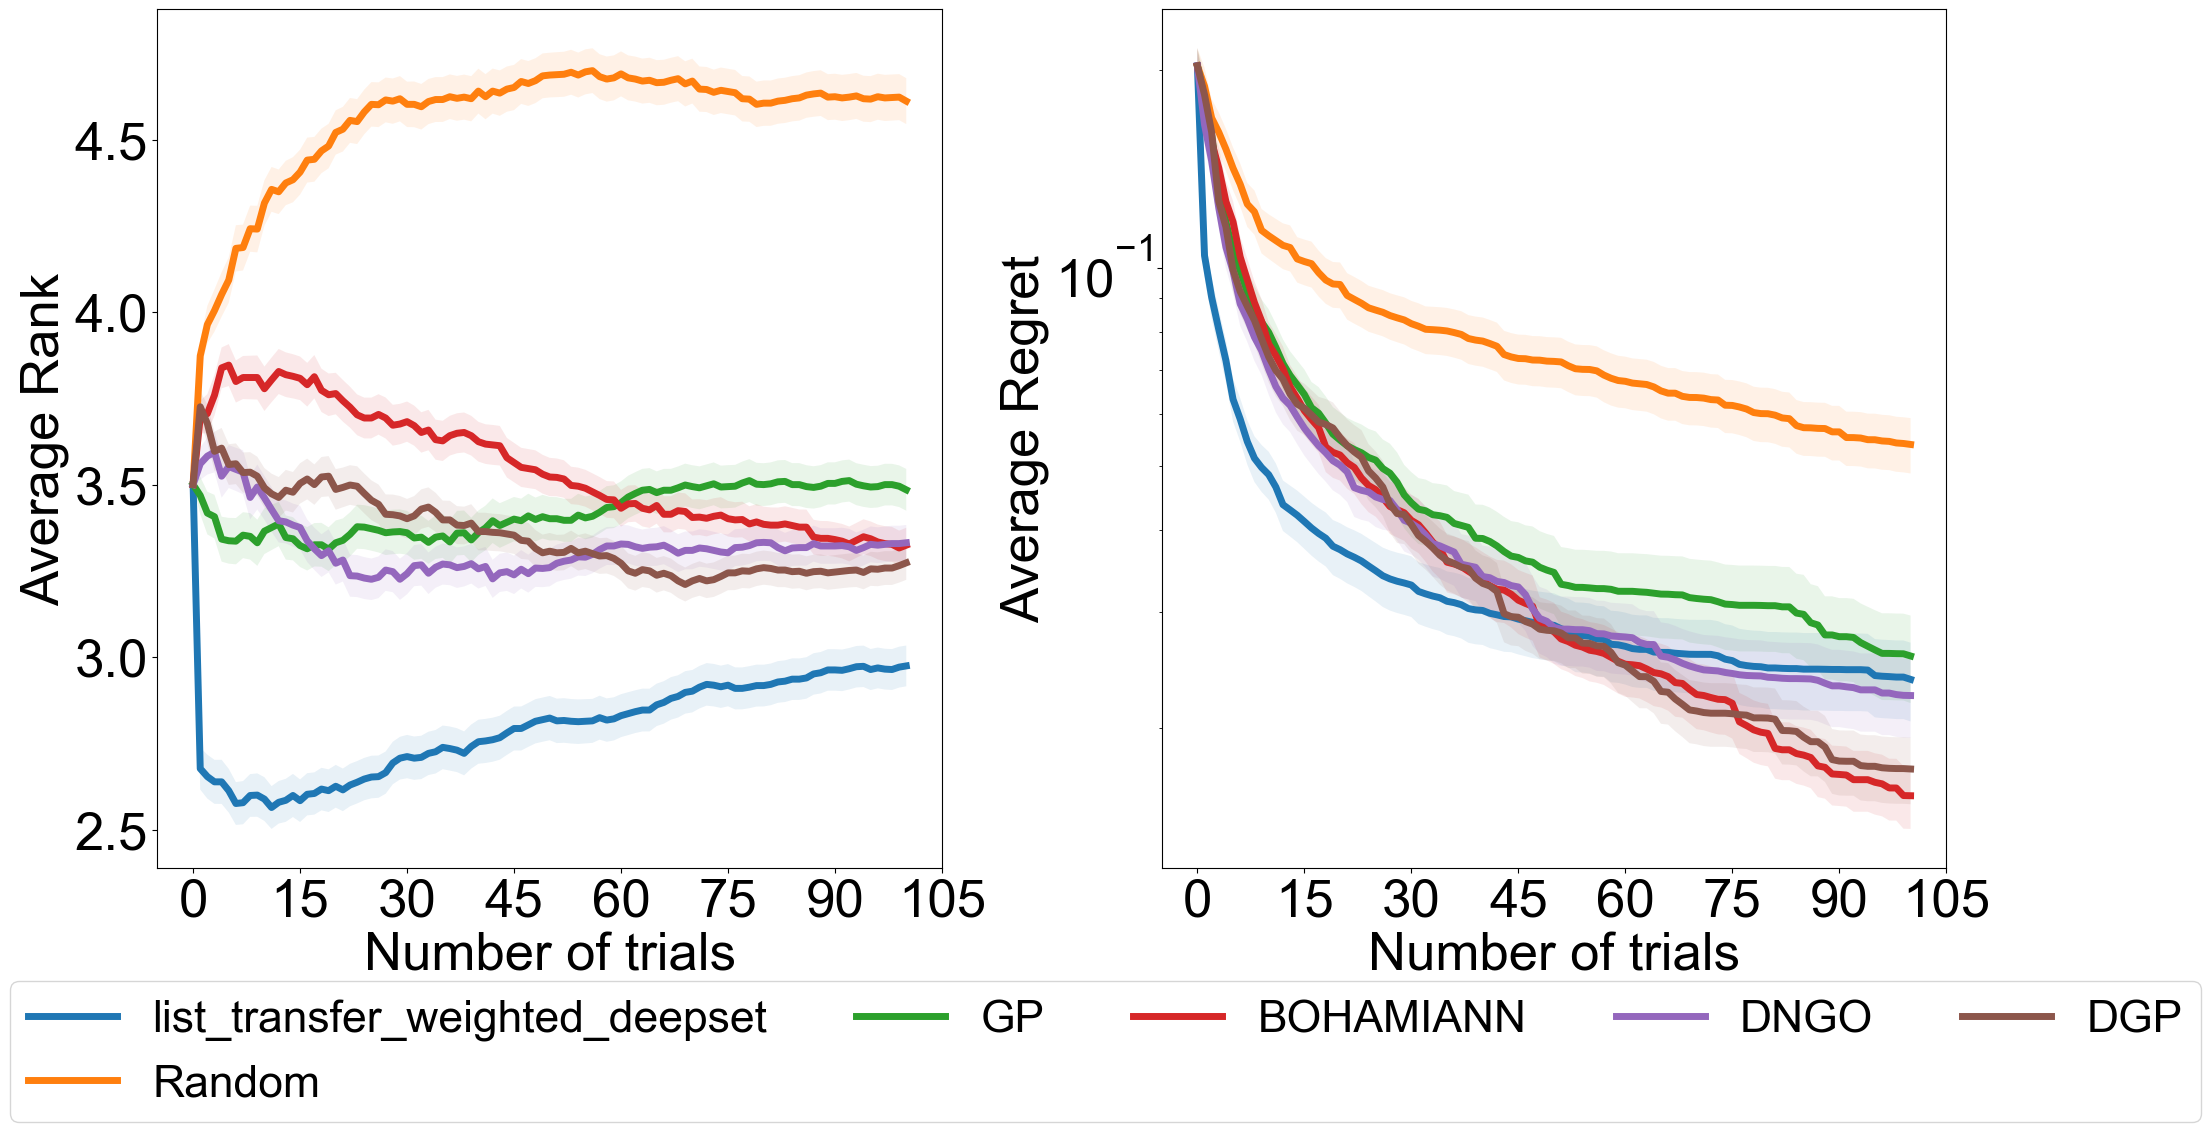
\includegraphics[scale=0.12]{images/NonTransferSOAT}
% \caption{Comparing the results of the proposed model against SOTA non-transfer HPO surrogates.}
    \label{fig:NonTransferSOTA}
\end{figure}


\begin{figure}[h]% [H] is so declass\'e!
\centering
\begin{minipage}{0.45\textwidth}
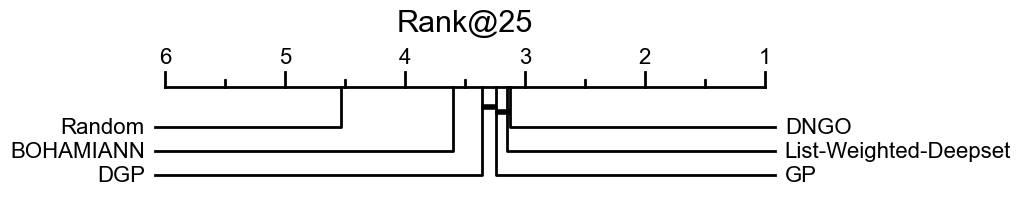
\includegraphics[width=\textwidth]{images/NonTransferSOTARank@25}
\end{minipage}\hfill
\begin{minipage}{0.45\textwidth}
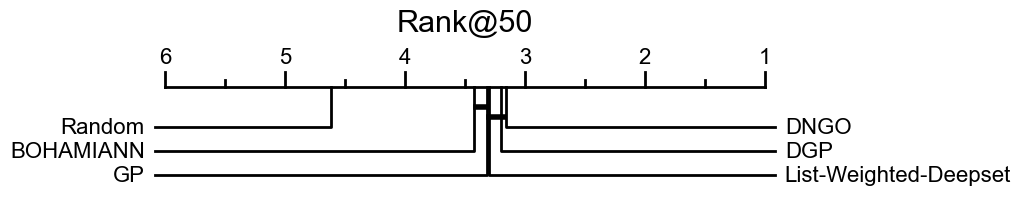
\includegraphics[width=\textwidth]{images/NonTransferSOTARank@50}
\end{minipage}\par
\vskip\floatsep% normal separation between figures
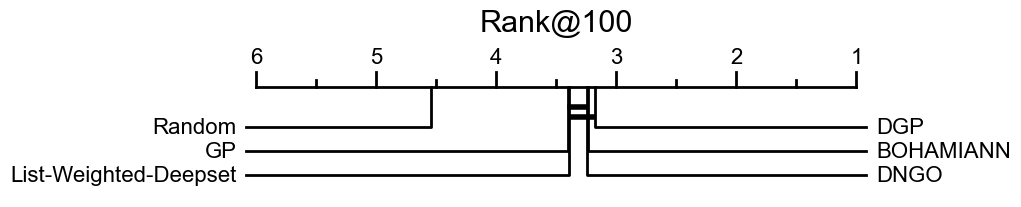
\includegraphics[width=0.45\textwidth]{images/NonTransferSOTARank@100}
    \caption{Graphs of the proposed model with other SOTA non-transfer HPO surrogates.}
   \label{fig:SOTANonTransferCriticalRankedGraph}
\end{figure}

\end{frame}


\begin{frame}[t]{Comparing with SOTA HPO models}
\textbf{Transfer HPO}

\begin{figure}[h]
  \centering
    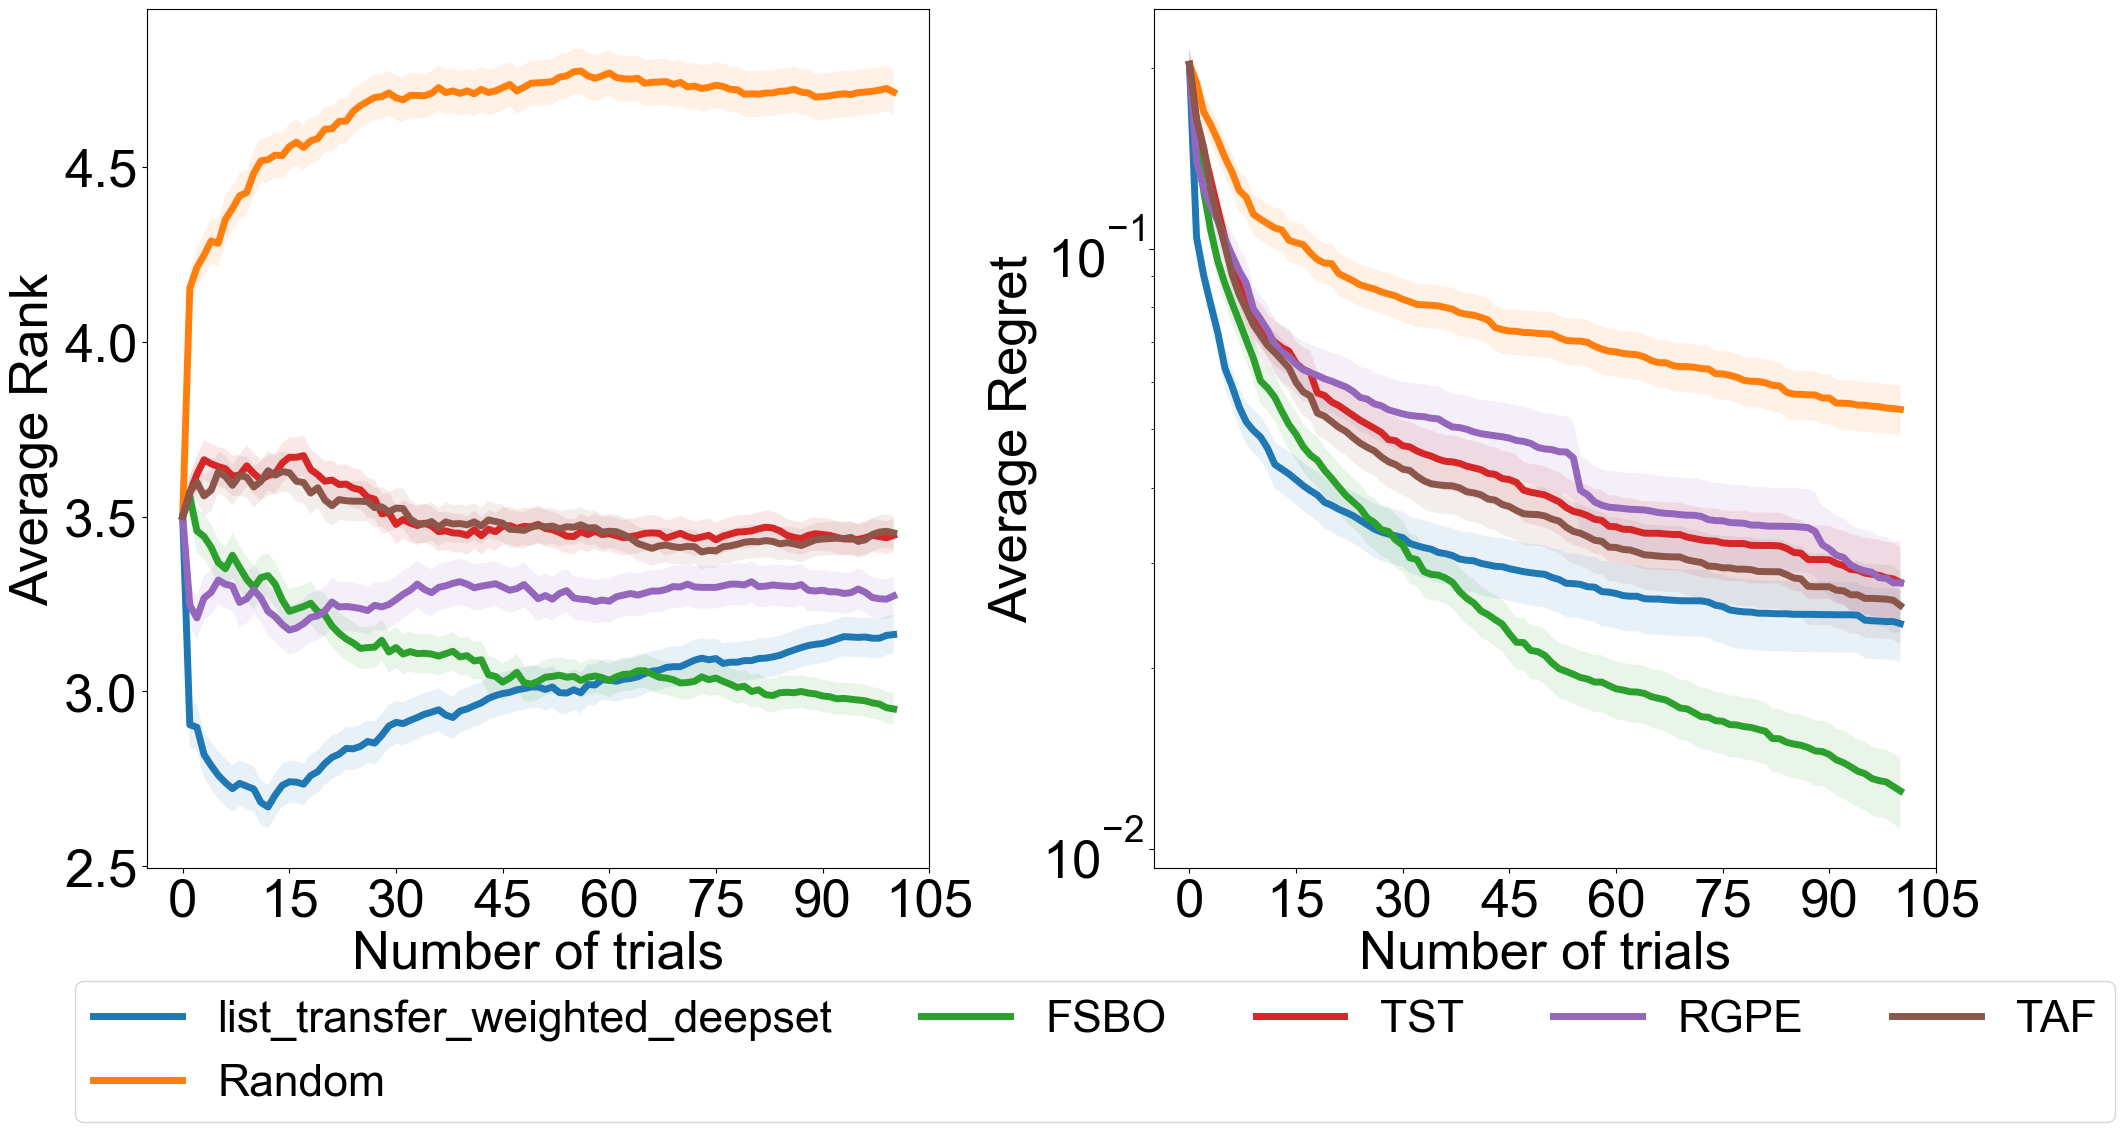
\includegraphics[scale=0.12]{images/TransferSOAT}
%    \caption{Comparing the results of the proposed model against SOTA transfer HPO surrogates.}
    \label{fig:TransferSOTA}
\end{figure}

\begin{figure}[h]% [H] is so declass\'e!
\centering
\begin{minipage}{0.45\textwidth}
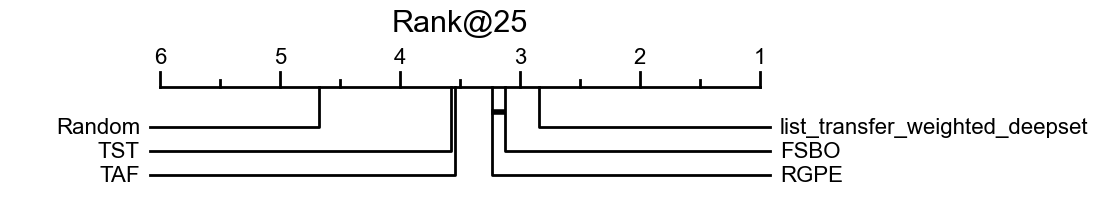
\includegraphics[width=\textwidth]{images/TransferSOATRank@25}
\end{minipage}\hfill
\begin{minipage}{0.45\textwidth}
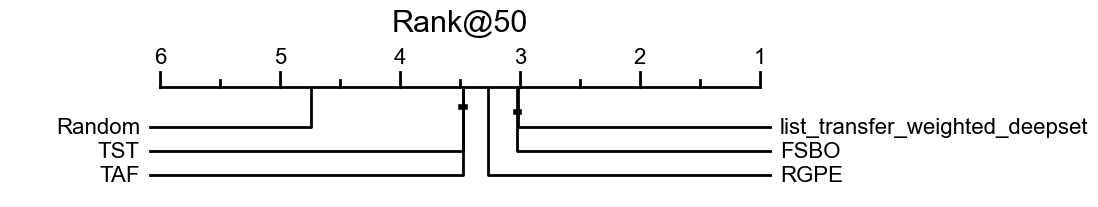
\includegraphics[width=\textwidth]{images/TransferSOATRank@50}
\end{minipage}\par
\vskip\floatsep% normal separation between figures
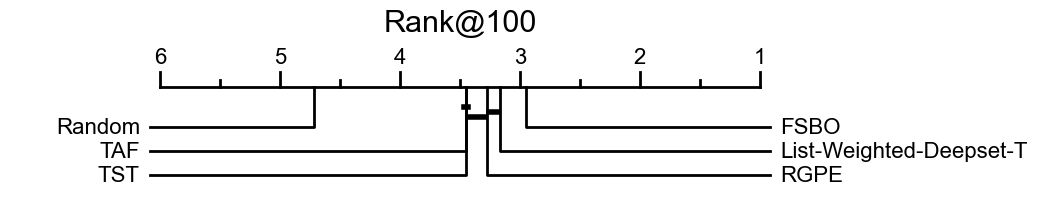
\includegraphics[width=0.45\textwidth]{images/TransferSOATRank@100}
   \caption{Graphs of the proposed model and SOTA transfer HPO surrogates.}
   \label{fig:SOTACriticalRankedGraph}
\end{figure}
\end{frame}

\begin{frame}[t]{Comparing with SOTA HPO models}
\textbf{Conclusion}
\begin{itemize}
\item Non transfer surrogate shows performance similar to the GP surrogate.
\item Transfer surrogate performance is on par with the state-of-the-art FSBO model.
\item Both transfer and non transfer version of the model perform very well in the initial evaluation steps.
\end{itemize}
\end{frame}

\section{Conclusion}
\begin{frame}
\centering
\LARGE{Conclusion}
\end{frame}

\begin{frame}[t]{Advantages and Limitations of the model.}
\textbf{Advantages}:
\begin{itemize}
\item Being a transfer HPO surrogate,  it utilises already existing meta data.
\item Sampling mechanism of listwise loss is superior.   For example,  from a set of 100 known HP configurations, there are ${100 \choose 15}$ ways to select a list of 15 items.
\item Working in ranking space dampens uncertainty. Slight noise in the HP evaluations does not change the ranks of the configurations.
\item Output ranges of HP evaluations across tasks do not affect the HP rankings.
\end{itemize}
\end{frame}

\begin{frame}[t]{Advantages and Limitations of the model.}
\textbf{Limitations}:
\begin{itemize}
\item We ignore the sorting functionality during the ranking loss formulation. Hence the complete ranking problem is not optimized.
\item We use exponentiation as the strictly increasing positive function. 
Hence there is a potential for overflow or underflow during optimization.
\item The learned surrogate may be biased towards tasks with lesser data due to the double sampling mechanism.
\item Negative transfer learning was seen in some search spaces.

\begin{figure}[htb]
  \centering
    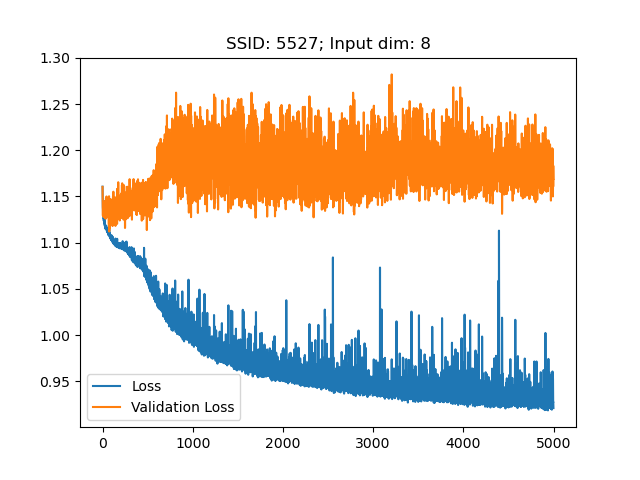
\includegraphics[scale=0.25]{images/NegativeLearning}
    \caption{Negative transfer learning example.}
    \label{fig:NegativeLearning}
\end{figure}

\end{itemize}
\end{frame}

\begin{frame}[t]{Further Research Directions}
\begin{itemize}
\item More research needs to be done for acquisition functions in the ranking space.
\item Study needs to be conducted to incorporate sorting functionality into the ranking loss. E.g., Using the model proposed by Swezey et al. ~\cite{PiRank}.
\item One could explore how to incorporate the learning mean and variance of the rank directly from the loss function instead of explicit calculation.
\item The proposed ranking surrogate only works in the discrete HP search space. We need to study how to incorporate this in the continuous HP Search Space.
\end{itemize}
\end{frame}

\begin{frame}[t]{Conclusion}
\begin{itemize}
\item The proposed model is an SMBO surrogate in the transfer HPO domain.
\item The study consisted of 2 canonical parts:
\begin{itemize}
\item Ranking loss functions
\item Surrogate design
\end{itemize}
\item Our results showed that listwise ranking losses perform the best compared to other losses.
\item After adding weighting \& Deep sets,  the surrogate performs comparably to FSBO (SOTA transfer HPO model).
\item \textbf{Key takeaway - For HPO,  working in the ranking space is better than the output space!}
\end{itemize}
\end{frame}

\section{Q \& A}

\begin{frame}
\centering
\LARGE{Q \& A}
\end{frame}

\section{References}

\begin{frame}[t]{References}

\begin{thebibliography}{1}

\bibitem{listmlepaper}
\alert{Xia et al.; Listwise approach to learning to rank: theory and algorithm (2008)}

\bibitem{ranknetpaper}
\alert{Burges et.  al; Learning to rank using gradient descent (2005)}

\bibitem{TRLWO}
\alert{Chen et.  al; Top-Rank Enhanced Listwise Optimization for Statistical Machine Translation (2017)}

\bibitem{subsetregressionpaper}
\alert{Cossock et. al ; Statistical Analysis of Bayes Optimal Subset Ranking (2008)}

\bibitem{fsbopaper}
\alert{Wistuba et.  al; Few-Shot Bayesian Optimization with Deep Kernel Surrogates (2021)}

\bibitem{successivehalving}
\alert{Jamieson et.  al;  Non-stochastic Best Arm Identification and Hyperparameter Optimization (2015)}

\end{thebibliography}

\end{frame}

\begin{frame}[t]{References}

\begin{thebibliography}{1}

\bibitem{DeepEnsemblesPaper}
\alert{Lakshminarayanan et al.; Simple and Scalable Predictive Uncertainty Estimation using Deep Ensembles (2017)}

\bibitem{PiRank}
\alert{Swezey et al.;  PiRank: Scalable Learning To Rank via Differentiable Sorting (2020).}

\end{thebibliography}

\end{frame}


\section{Appendix}
\begin{frame}
\centering
\LARGE{Appendix}
\end{frame}

\iffalse
\section{Surrogate usage with HPO-B Benchmark}
\begin{frame}
\centering
\LARGE{Surrogate Usage in HPO-B Benchmark}
\end{frame}
\fi

\begin{frame}[t]{UCB and EI in the ranking space}
\begin{itemize}
\item Experiments in our study used the average rank acquisition function.
\item Here, we integrate UCB (Upper Confidence Bound) and EI (Expected Improvement) in the ranking space.
\item UCB is calculated using the mean and standard deviations returned from the ensemble of rankers.
\item EI is calculated by passing the HP incumbent in both the query and the support set.
\item Comparison is made between Average-Rank,  UCB-Rank,  EI-Rank, and all the transfer HPO models.
\item \textbf{Conclusion}:
\begin{itemize}
\item UCB and EI acquisition functions are superior even in the ranking space. \item The proposed surrogate model with EI  acquisition function performs better than FSBO in all optimization steps.
\end{itemize}
\end{itemize}
\end{frame}

\begin{frame}[t]{UCB and EI in the Ranking space}
\begin{figure}[h]
  \centering
    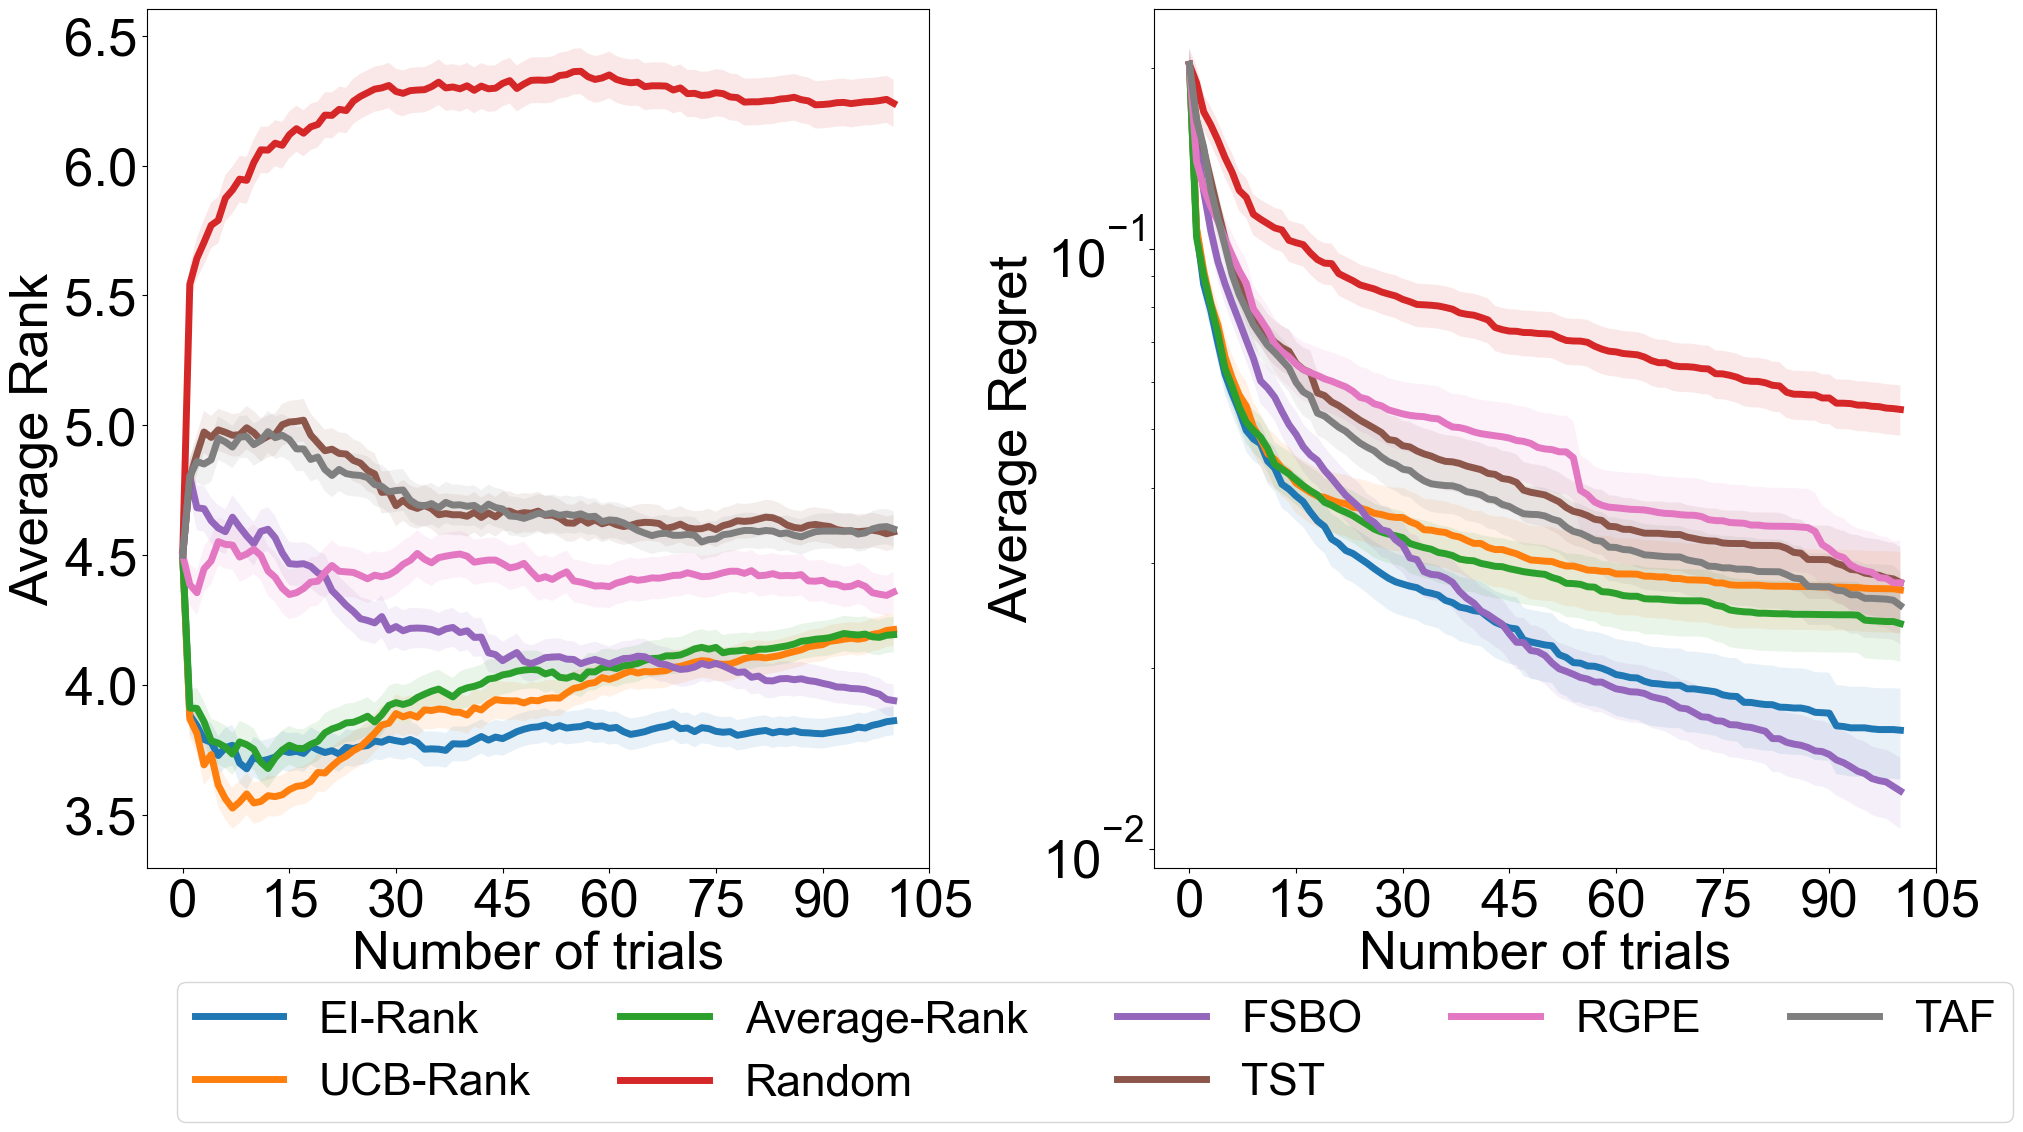
\includegraphics[scale=0.20]{images/acqusitionRanking}
    \caption{Ablation of Average-Rank, UCB-Rank, and EI-Rank with other SOTA transfer HPO methods.}
    \label{fig:acqusitionRanking}
\end{figure}

\end{frame}

\begin{frame}[t]{HPO-B Benchmark}
\begin{figure}[htb]
\centering
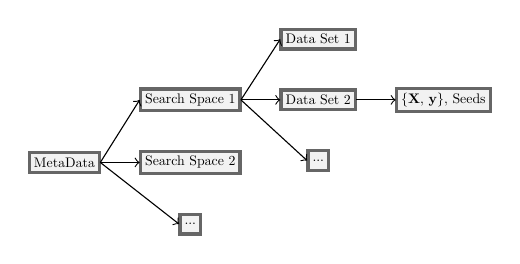
\begin{tikzpicture}[scale=0.5, transform shape,
% roundnode/.style={circle, draw=green!60, fill=green!5, very thick, minimum size=7mm},
squarednode/.style={rectangle, draw=black!60, fill=black!5, very thick, minimum size=5mm},
]
%Nodes
\node[squarednode]      (ss2)                             {Search Space 2};
\node[squarednode]      (main)                   [left=of ss2]           {MetaData};
\node[squarednode]      (ss1)                    [above=of ss2]          {Search Space 1};
\node[squarednode]      (ss_)                       [below=of ss2]        {...};
\node[squarednode]      (ds2)                       [right=of ss1]        {Data Set 2};
\node[squarednode]      (ds1)                       [above=of ds2]        {Data Set 1};
\node[squarednode]      (ds_)                       [below=of ds2]        {...};
\node[squarednode]      (Xy)                       [right=of ds2]        {\{\textbf{X},  \textbf{y}\},  \textrm{Seeds}};

%Lines
\draw[->] (main.east) -- (ss2.west);
\draw[->] (main.east) -- (ss1.west);
\draw[->] (main.east) -- (ss_.west);
\draw[->] (ss1.east) -- (ds2.west);
\draw[->] (ss1.east) -- (ds1.west);
\draw[->] (ss1.east) -- (ds_.west);
\draw[->] (ds2.east) -- (Xy.west);
\end{tikzpicture}
\caption{Structure of the metadata in the HPO-B benchmark.}
\label{fig:metadataorganization}
\end{figure}

\begin{itemize}
\item HPO-B is used for benchmarking BlackBox HPO.
\item It consists of multiple Search Spaces (SS). An SS signifies a single ML model.
\item Each SS consists of different Data Sets.
\item A Data Set (task) contains HP configurations \& their\\
evaluations for a single training instance of the model.
\item Seeds specify different initial configurations to start the \\
SMBO process.
\end{itemize}
\end{frame}

\end{document}


